\chapter{Methodology}
\label{cha:methodology}

The observed-data log-likelihood under the model of Chapter~\ref{cha:model-specification} is

\begin{equation}
    l(\bm{\theta})=\sum_{j=1}^{J}\sum_{i\in \mathcal{I}_{j}}\log p(\bm{y}_{ij}\mid \bm{\theta})=\sum_{j=1}^{J}\sum_{i\in \mathcal{I}_{j}}\log \int p(\bm{y}_{ij}\mid \bm{\lambda}_{j})p(\bm{\lambda}_{j}\mid \bm{\Sigma})\,d\bm{\lambda}_{j},
    \label{eq:log-lik-chap2}
\end{equation}

where the parameter space is $\bm{\theta}:=\{\bm{\mu}, \bm{\Phi}, \mathbf{B},\sigma^{2}\}$. The integral in \eqref{eq:log-lik-chap2} has no closed form, because the Gaussian prior on $\bm{\lambda}_{j}$ is not conjugate to the multinomial likelihood, so we treat $\{\bm{\lambda}_{j}\}_{j=1}^{J}$ as missing data and then estimate $\bm{\theta}=\{\bm{\mu}, \bm{\Phi}, \mathbf{B},\sigma^{2}\}$ by EM. The standard approach in generalized linear mixed models is the Laplace approximation (\citep{Breslow1993}, \citep{Tierney1986}), which replaced the integral with a Gaussian approximation at the posterior mode.

\iffalse
\section{The Choice of Approximation Level}
\label{sec:the-choice-of-approximation-level}

A natural approach motivated by \citet{Chiquet2018} and their PLN-PCA model approximates the posterior of the K-dimensional factor $p(\mathbf{f}_{j}\mid \bm{y}_{ij})$, which was adapted by \citet{mcgillycuddy2024} in their latent model structure. Since we assumed $K\ll Q$, this reduces the Newton-step Hessian from $Q\times Q$ to $K\times K$, which appears computationally attractive. However, this approach encounters two fundamental obstacles. 

\paragraph*{Group Collapsing} Within group $j$, observations $\{i\in \mathcal{I}_{j}\}$ share the same factor $\mathbf{f}_{j}$ but carry distinct covariate vectors $\bm{v}_{ij}$ and total count $y_{ij\cdot}$. The factor-space log-posterior requires summing $\sum_{i\in \mathcal{I}_{j}}\log p(\bm{y}_{ij}\mid \mathbf{f}_{j})$, where each term involves its own normalizing constant $\sum_q \exp\bigl(\eta_{ijq}(\mathbf{f}_j)\bigr)$. A naive implementation collapses all observations in group $j$ into a single super-observation with total counts $\bm{y}_{\cdot j} = \sum_{i\in \mathcal{I}_{j}} \bm{y}_{ij}$ and averaged fixed effects $\bar{\bm{\eta}}_{j}$, treating the group as a single Multinomial draw. This is mathematically incorrect. The Multinomial log-normalizer does not linearize under summation, and the approximation error grows with within-group heterogeneity in $\bm{v}_{ij}$. 

\paragraph*{Posterior Second-Moment Deflation} The factor-space Laplace posterior yields a second-moment matrix $\mathbf{W}_{f}=J^{-1}\sum_{j}(\hat{\mathbf{f}}_{j}\hat{\mathbf{f}}_{j}^{\top}+\hat{\mathbf{V}}_{j})$ that systematically underestimates $\mathbf{I}_{K}$ due to Laplace shrinkage. Because the M-step for $\mathbf{B}$ receives only $\mathbf{BW}_{f}\mathbf{B}^{\top}$ as its sufficient statistic for $\bm{\Sigma}$, the Rubin–Thayer algorithm (\citet{Rubin1982}) compensates by inflating $\hat{\mathbf{B}}$, leading to the error in estimation. 
Thus, instead of approximate the posterior of $K$ dimensional latent factors, we do the approximation on Q dimensional group random effect $p(\bm{\lambda}_{j}\mid \bm{y}_{ij})$ directly and move the factor decomposition from the E-step to the M-step. The E-step treats $\bm{\lambda}_{j}$ as an unknown Q-vector with Gaussian prior $\mathcal{N}(\bm{0},\bm{\Sigma})$, then the M-step decomposes the resulting estimated covariance $\hat{\bm{\Sigma}}_{\text{obs}}$ into $\mathbf{BB}^{\top}+\sigma^{2}\mathbf{I}$.

Before we lay out our detailed EM algorithm, we introduce three technical conditions, which will significantly simplify our presentation. Different from single scalar space, our parameter space $\bm{\theta}=\{\bm{\mu}, \bm{\Phi}, \mathbf{B},\sigma^{2}\}$ given by~\eqref{eq:log-lik-chap2} contains both scalar, vector and matrix.

\begin{condition}[Self-Consistency]
Function $Q(\cdot\mid \bm{\theta^{*}})$ is self-consistency, namely
\begin{equation}
    \bm{\theta^{*}}=\arg\max_{\bm{\theta}\in \Omega} Q(\bm{\theta}\mid \bm{\theta^{*}})
    \label{eq:self-consistency}
\end{equation}
\end{condition}

\begin{condition}[Strong Concavity and Smoothness]
$Q(\cdot\mid \bm{\theta^{*}})$ is strongly concave over $\Omega$, that is,
\begin{equation}
    Q(\bm{\theta}_{2}\mid \bm{\theta^{*}})-Q(\bm{\theta}_{1}\mid \bm{\theta^{*}})-\langle \nabla Q(\bm{\theta}_{1}\mid \bm{\theta^{*}}), \bm{\theta}_{2}-\bm{\theta}_{1}\rangle\leq -\frac{\gamma}{2}\|\bm{\theta}_{2}-\bm{\theta}_{1}\|^{2}, \quad \forall \bm{\theta}_{1},\bm{\theta}_{2}\in \Omega.
    \label{eq:strong-concave}
\end{equation}
$Q(\cdot\mid \bm{\theta^{*}})$ is $\mu$-smooth over $\Omega$, that is, for any $\bm{\theta}$ near $\bm{\theta}^{*}$,
\begin{equation}
    Q(\bm{\theta}_{2}\mid \bm{\theta^{*}})-Q(\bm{\theta}_{1}\mid \bm{\theta^{*}})-\langle \nabla Q(\bm{\theta}_{1}\mid \bm{\theta^{*}}), \bm{\theta}_{2}-\bm{\theta}_{1}\rangle\geq -\frac{\mu}{2}\|\bm{\theta}_{2}-\bm{\theta}_{1}\|^{2}, \quad \forall \bm{\theta}_{1},\bm{\theta}_{2}\in \Omega.
    \label{eq:smooth}
\end{equation}
\end{condition}

\begin{condition}[Gradient Stability]
    \begin{equation}
        \| \nabla Q(\mathcal{M}(\bm{\theta})\mid \bm{\theta})-\nabla Q(\mathcal{M}(\bm{\theta})\mid \bm{\theta}^{*})\|\leq \tau \|\bm{\theta}-\bm{\theta}^{*}\|
    \end{equation}
\end{condition}
\fi

\section{EM Algorithm \& Convergence}
\label{sec: EM}
    For each group $j$, the log-posterior of $\bm{\lambda}_{j}$ is given by:
\begin{equation}
    \ell(\bm{\lambda}_{j})=\sum_{i\in \mathcal{I}_{j}}\Bigl[\sum_{q}y_{ijq}\eta_{ijq}(\bm{\lambda}_{j})-y_{ij\cdot}\log \sum_{q}\exp\bigl(\eta_{ijq}(\bm{\lambda}_{j})\bigr)\Bigr]-\frac{1}{2}\bm{\lambda}_{j}^{\top}\bm{\Sigma}^{-1}\bm{\lambda}_{j},
    \label{eq: estep-loglik}
\end{equation}
up to an additive constant independent of $\bm{\lambda}_{j}$, where 
\begin{equation}
    \eta_{ijq}(\bm{\lambda}_{j})=\mu_{q}+\bm{v}_{ij}^{\top}\bm{\phi}_{q}+\lambda_{jq},
    \label{eq: individualcovariate}
\end{equation}
is evaluated separately for each $i\in \mathcal{I}_{j}$, gives the individual-specific covariate structure.
The gradient and Hessian of \eqref{eq: estep-loglik} are

\begin{equation}
    \nabla_{\bm{\lambda}_{j}}\ell=\sum_{i\in \mathcal{I}_{j}}\bigl(\bm{y}_{ij}-y_{ij\cdot}\bm{p}_{ij}(\bm{\lambda}_{j})\bigr)-\bm{\Sigma}^{-1}\bm{\lambda}_{j},
\end{equation}

\begin{equation}
    \mathbf{H}(\bm{\lambda}_{j})=-\sum_{i\in\mathcal{I}_{j}}y_{ij\cdot}\left(\text{diag}(\bm{p}_{ij})-\bm{p}_{ij}\bm{p}_{ij}^{\top}\right)-\bm{\Sigma}^{-1},
    \label{eq: hessian-equality}
\end{equation}
where $\bm{p}_{ij}(\bm{\lambda}_{j})=\operatorname{softmax}\bigl(\bm{\eta}_{ij}(\bm{\lambda}_{j})\bigr)$. Since $\mathbf{P}_{ij}\succeq 0$ and $\bm{\Sigma}^{-1}\succ 0$, we have $\mathbf{H}(\bm{\lambda}_{j})\prec 0$ everywhere, so $\ell(\bm{\lambda}_{j})$ is strictly concave and has a unique maximizer

\begin{equation}
     \hat{\bm{\lambda}}_{j}
     = \arg\max_{\bm{\lambda}\in \mathbb{R}^{Q}}
     \ell_{j}(\bm{\lambda}_{j}),
     \label{eq:maximizer}
\end{equation}
which can be found by Newton's method with Armijo backtracking search with step size $s^{(t)}\in (0,1]$. Strict concavity guarantees convergence to $\hat{\bm{\lambda}}_{j}$ from any starting point. The Laplace approximation then replaces the intractable posterior with the Gaussian matched to the model and curvature at,

\begin{equation}
    \bm{\lambda}_{j}^{(t+1)}=
    \bm{\lambda}_{j}^{(t)}
    -s^{(t)}\mathbf{H}\bigl(\bm{\lambda}_{j}^{(t)}
    \bigr)^{-1}\nabla_{\bm{\lambda}_{j}}
    \ell \bigl(\bm{\lambda}_{j}^{(t)}\bigr),
    \label{eq:newton-method}
\end{equation}
with backtracking step size $s^{(t)}$ converges to the unique global maximum $\hat{\bm{\lambda}}_{j}$ from any initialization. The Laplace approximation then yields

\begin{equation}
    p(\bm{\lambda}_{j}\mid \bm{y}_{ij}) \approx \mathcal{N}\bigl(\hat{\bm{\lambda}}_{j}, \hat{\mathbf{S}}_{j}\bigr), \quad \hat{\mathbf{S}}_{j}=\bigl(-\mathbf{H}(\hat{\bm{\lambda}_{j}})\bigr)^{-1}.
    \label{eq:surrogate-eq}
\end{equation}

Each Newton step requires forming and solving the $Q\times Q$ system in \eqref{eq: hessian-equality} at a cost of $\mathcal{O}(I_{j}Q^{2}+Q^{3})$ per step. We will discuss and remove this bottleneck in Chapter~\ref{cha:computational-acceleration}.


With $\hat{\bm{\lambda}}_{j}$ fixed, recompute the Poisson-Multinomial Equivalence offset:
\begin{equation}
    \xi_{ij}=\log y_{ij\cdot}-\log \sum_{q}\exp\bigl(\hat{\mu}_{q}+\bm{v}_{ij}^{\top}\hat{\bm{\phi}}_{q}+\hat{\lambda}_{jq}\bigr).
\end{equation}
For $q=1,2,\dots,Q$, we solve the maximization problem independently:
\begin{equation}
    (\hat{\mu}_{q}, \hat{\bm{\phi}}_{q})=\arg \max_{\mu_{q}, \bm{\phi}_{q}}\sum_{i}\bigl[y_{ijq}(\mu_{q}+\bm{v}_{ij}^{\top}\bm{\phi}_{q})-\exp (\mu_{q}+\bm{v}_{ij}^{\top}\bm{\phi}_{q}+\hat{\lambda}_{jq}+\xi_{ij})\bigr].
\end{equation}
This is a Poisson log-linear regression with offset $\lambda_{jq}+\xi_{ij}$, solved by iteratively reweighted least squares. The Q problems are independent and may be parallelized. 

The EM sufficient statistic for $\bm{\Sigma}$ follows directly from the Laplace output:

\begin{equation}
    \hat{\bm{\Sigma}}_{\text{obs}}=\frac{1}{J}\sum_{j}\mathbb{E}[\bm{\lambda}_{j} \bm{\lambda}_{j}^{\top}\mid \bm{y}_{ij}]\approx \frac{1}{J}\sum_{j}(\hat{\bm{\lambda}}_{j} \hat{\bm{\lambda}}_{j}^{\top}+\hat{\mathbf{S}}_{j}).
    \label{eq:sigma-obs}
\end{equation}

Critically, $\hat{\bm{\Sigma}}_{\text{obs}}$ is fully determined by current Laplace output $(\hat{\bm{\lambda}}_{j}, \hat{\mathbf{S}}_{j})$ and does not need to be re-evaluated during the Rubin-Thayer sub-iterations, thus eliminating the circular dependency inherent in factor-space formulations.
Given $\hat{\bm{\Sigma}}_{\text{obs}}$, we decompose $\bm{\Sigma}=\mathbf{BB}^{\top}+\sigma^2\mathbf{I}_{Q}$ via the Rubin-Thayer EM factor analysis algorithm (\citet{Rubin1982})

\begin{equation}
\hat{\boldsymbol{\beta}}
=
\hat{\mathbf{B}}^\top
\left(
\hat{\mathbf{B}}\hat{\mathbf{B}}^\top
+
\hat{\sigma}^2 \mathbf{I}_Q
\right)^{-1},
\label{eq: Rubin1}
\end{equation}
\begin{equation}
\hat{\boldsymbol{\Theta}}
=
\mathbf{I}_{K}
-
\hat{\boldsymbol{\beta}}\hat{\mathbf{B}}
+
\hat{\boldsymbol{\beta}}
\hat{\boldsymbol{\Sigma}}_{\mathrm{obs}}
\hat{\boldsymbol{\beta}}^\top,
\label{eq: Rubin2}
\end{equation}
\begin{equation}
\hat{\mathbf{B}}_{\mathrm{new}}
=
\hat{\boldsymbol{\Sigma}}_{\mathrm{obs}}
\hat{\boldsymbol{\beta}}^\top
\hat{\boldsymbol{\Theta}}^{-1},
\label{eq: Rubin3}
\end{equation}
\begin{equation}
\hat{\sigma}_{\mathrm{new}}^{2}
=
\frac{1}{Q}
\operatorname{tr}
\left(
\hat{\boldsymbol{\Sigma}}_{\mathrm{obs}}
-
\hat{\mathbf{B}}_{\mathrm{new}}
\hat{\boldsymbol{\beta}}
\hat{\boldsymbol{\Sigma}}_{\mathrm{obs}}
\right).
\label{eq: Rubin4}
\end{equation}

The iterations  \eqref{eq: Rubin1}-\eqref{eq: Rubin4} are repeated to convergence. The PLT constraint is enforced post-hoc via a QR decomposition of the top K rows of $\hat{\mathbf{B}}_{\text{new}}$, followed by sign correction to ensure positive diagonal entries and zeroing of the upper triangle. Applying PLT only after the Rubin–Thayer sub-iterations converge, rather than at each inner step, avoids the discontinuities that would otherwise disrupt convergence.
    Given $\hat{\mathbf{B}}$ and $\hat{\sigma}^2$, the factor scores are recovered by the Bayes linear estimator \citep{Gelman2013}:
\begin{equation}
\hat{\mathbf{f}}_j = \left( \mathbf{I}_K + \frac{1}{\hat{\sigma}^2} \hat{\mathbf{B}}^\top \hat{\mathbf{B}} \right)^{-1} \frac{1}{\hat{\sigma}^2} \hat{\mathbf{B}}^\top \hat{\boldsymbol{\lambda}}_j ,
\label{eq: Bayeslinearestimator}
\end{equation}
requiring only $K\times K$ inversion.

Chapter~\ref{cha:methodology} derived a correct and convergent Laplace-EM algorithm, but left its dominant per-iteration cost unaddressed. Each Newton step in E-step requires forming and solving the $Q\times Q$ system~\eqref{eq: hessian-equality} at cost $\mathcal{O}(I_{j}Q^{2}+Q^{3})$, in the meanwhile, each inner iteration of the M-step factor update~\eqref{eq: Rubin3}-\eqref{eq: Rubin4} requires forming $\bm{\Sigma}^{-1}$ densely at cost $\mathcal{O}(Q^{3})$. For large Q, these costs are not merely inconvenient but make the algorithm impractical. This chapter develops an exact acceleration method to remove this bottleneck by showing that the Poisson-Multinomial equivalence that already underlies the M-step can be redeployed via auxiliary-variable construction, which can remove the cross-category coupling from the E-step Hessian as well. 

\section{Three Methods for Rate \& Accuracy}

\subsection{PME Auxiliary-Variable Construction \& Woodbury Solve}
\label{subsec:auxiliary-variable-construction}

Indirect inference (II) is a methodology for estimating the parameters of an intractable (generative) model on the basis of an alternative parametric (auxiliary) model that is both analytically and computationally easier to deal with. \citet{Drovandi2015} introduced the parametric Bayesian indirect inference (pBII) methods 

For a fixed group $j$, we introduce an auxiliary scalar $\xi_{i}$ per observation $i\in \mathcal{I}_{j}$ and define the Poisson surrogate log-posterior
\begin{equation}
    \ell_P(\boldsymbol{\lambda}, \boldsymbol{\xi}) \;=\; \sum_{i \in \mathcal{I}_j} \sum_{q=1}^{Q} \Big[ y_{iq}\, \eta_{iq}(\boldsymbol{\lambda}) - \exp\big(\eta_{iq}(\boldsymbol{\lambda}) + \xi_i\big) \Big] \;-\; \tfrac{1}{2} \boldsymbol{\lambda}^\top \boldsymbol{\Sigma}^{-1} \boldsymbol{\lambda},
\end{equation}
which treats the counts as independent Poisson draws with rate $\exp{(\eta_{iq}+\xi_{i})}$ rather than as a multinomial draw. This is the same auxiliary-variable idea, but it is now applied to the E-step posterior instead of M-step likelihood.

With $\bm{\xi}$ fixed at $\bm{\xi}^{*}(\bm{\lambda})$, we denote $d_{q}:=\sum_{i\in \mathcal{I}_{j}}\exp{\bigl(\eta_{iq}(\bm{\lambda})+\xi_{i}\bigr)}$. The Hessian of $\ell_{P}(\cdot, \bm{\xi})$ with respect to $\bm{\lambda}$ is 
\begin{equation}
    \mathbf{H}_{P}(\bm{\lambda})=-\text{diag}(\mathbf{d})-\bm{\Sigma}^{-1}, \quad \mathbf{d}=(d_{1},\dots, d_{Q})^{\top},
    \label{eq:acceleration-hessian1}
\end{equation}
which is purely diagonal in its Poisson part. We expand $\bm{\Sigma}^{-1}$ by the Woodbury identity

\begin{equation}
    \bm{\Sigma}^{-1}=\sigma^{-2}\mathbf{I}_{Q}-\sigma^{-4}\mathbf{BM}_{K}^{-1}\mathbf{B}^{\top} \text{ with } \mathbf{M}_{K}=\mathbf{I}_{K}+\sigma^{-2}\mathbf{B}^{\top}\mathbf{B}.
    \label{eq:woodbury2}
\end{equation}

We write $\tilde{\mathbf{D}}=\text{diag}(\mathbf{d}+\sigma^{-2}\mathbf{1}_{Q})$ for the combined diagonal term
\begin{equation}
    -\mathbf{H}_{P}(\bm{\lambda})=\tilde{\mathbf{D}}-\sigma^{-4}\mathbf{BM}_{K}^{-1}\mathbf{B}^{\top},
    \label{eq:acceleration-hessian3}
\end{equation}
it's a $Q\times Q$ matrix. Applying Woodbury identity once more and we obtain
\begin{equation}
    \bigl(-\mathbf{H}_{P}(\bm{\lambda})\bigr)^{-1}=\tilde{\mathbf{D}}^{-1}-\tilde{\mathbf{D}}^{-1}\mathbf{B}\bm{\Gamma}^{-1}\mathbf{B}^{\top}\tilde{\mathbf{D}}^{-1} \text{ with } \bm{\Gamma}:=\mathbf{B}^{\top}\tilde{\mathbf{D}}^{-1}\mathbf{B}-\sigma^{4}\mathbf{M}_{K}.
    \label{eq:inverse-hessian4}
\end{equation}

Therefore, given the Cholesky factor $\mathbf{L}$ of $-\bm{\Gamma}$, a Newton direction $\Delta\bm{\lambda}=\bigl(-\mathbf{H}_{P}(\bm{\lambda})\bigr)^{-1}\mathbf{g}$ for any gradient vector $\mathbf{g}$ is obtained as

\begin{equation}
    \Delta\boldsymbol{\lambda} \;=\; \tilde{\mathbf{D}}^{-1}\mathbf{g} \;+\; \tilde{\mathbf{D}}^{-1}\mathbf{B}(\mathbf{L}\mathbf{L}^\top)^{-1}\mathbf{B}^\top\tilde{\mathbf{D}}^{-1}\mathbf{g},
    \label{eq:newton-direction5}
\end{equation}
computed by two matrix-vector products against $\mathbf{B}$ and one $K\times K$ triangular solve, after a one-time $\mathcal{O}(QK^{2}+K^{3})$ cost to form $\bm{\Gamma}$ and its Cholesky factor.

\begin{proposition}[Negative definiteness and conditioning of $\bm{\Gamma}$]
    If $\bm{\Gamma}\prec 0$ and $\lambda_{\text{max}}(\bm{\Gamma})\leq -\sigma^{4}$, then $-\bm{\Gamma}\succ \sigma^{4}\mathbf{I}_{K}$ uniformly in $\bm{\lambda}$, $\mathbf{B}$ and data.
    \label{prop:negative-definiteness}
\end{proposition}

\begin{proof}
    Since $d_{q}\geq 0$ for each $q$, $\tilde{\mathbf{D}}=\text{diag}(\mathbf{d}+\sigma^{-2}\mathbf{1}_{Q})\succeq \sigma^{-2}\mathbf{I}_{Q}$. Therefore, $\tilde{\mathbf{D}}^{-1}\preceq \sigma^{2}\mathbf{I}_{Q}$ and $\mathbf{B}^{\top}\tilde{\mathbf{D}}^{-1}\mathbf{B}\preceq \sigma^{2}\mathbf{B}^{\top}\mathbf{B}$.
    Rewrite the definition of $\bm{\Gamma}$ in~\eqref{eq:inverse-hessian4} using the substitution $\mathbf{M}_{K}=\mathbf{I}_{K}+\sigma^{-2}\mathbf{B}^{\top}\mathbf{B}$, then
    \[
        -\bm{\Gamma}=\sigma^{4}\mathbf{M}_{K}-\mathbf{B}^{\top}\tilde{\mathbf{D}}^{-1}\mathbf{B}\succeq \sigma^{4}\mathbf{M}_{K}+\sigma^{2}\mathbf{B}^{\top}\mathbf{B}-\sigma^{2}\mathbf{B}^{\top}\mathbf{B}=\sigma^{4}\mathbf{I}_{K}.
    \]
\end{proof}

Proposition~\ref{prop:negative-definiteness} guarantees that the Cholesky factorization used in~\eqref{eq:newton-direction5} is always numerically well behaved. Regardless of how large $Q$ and $\mathbf{B}$ increase, the relevant $K\times K$ matrix never becomes ill-conditioned purely as an artefact of dimension, since its smallest eigenvalue is bounded below by the dimension-free quantity $\sigma^{4}$.

The direction $\Delta \bm{\lambda}$ of~\eqref{eq:newton-direction5} is a Newton step for the surrogate objective $\ell_{P}(\cdot, \bm{\xi}^{*}\bigl(\bm{\lambda})\bigr)$ instead of true log-posterior $\ell$.

\begin{algorithm}[t]
    \caption{E-step inner iteration: posterior-mode search for the group effect $\bm{\lambda}_j$}
    \label{alg:estep-inner}
    \begin{algorithmic}[1]
    \Require group data $\{\bm{y}_{ij}\}_{i\in\mathcal{I}_j}$; current parameters
         $(\bm{\mu},\bm{\Phi},\mathbf{B},\sigma^2)$; Armijo constants
         $c_1\in(0,1)$, $\rho\in(0,1)$; tolerance $\epsilon>0$
    \Ensure posterior mode $\widehat{\bm{\lambda}}_j$ and curvature $-\mathbf{H}(\widehat{\bm{\lambda}}_j)$
    \State initialize $\bm{\lambda}^{(0)}\gets \mathbf{0}$;\quad $t\gets 0$
    \Repeat
    \State re-profile the offset $\bm{\xi}^{(t)}\gets \bm{\xi}(\bm{\lambda}^{(t)})$
    \State $\mathbf{g}^{(t)}\gets \nabla\ell(\bm{\lambda}^{(t)})$
    \State form $-\mathbf{H}_P(\bm{\lambda}^{(t)})
         =\bar{\mathbf{D}}^{(t)}-\sigma^{-4}\mathbf{B}\mathbf{M}_K^{-1}\mathbf{B}^\top$
    \State solve $\bigl(-\mathbf{H}_P(\bm{\lambda}^{(t)})\bigr)\,\Delta\bm{\lambda}^{(t)}=\mathbf{g}^{(t)}$
    \State $s^{(t)}\gets 1$
    \While{$\ell\bigl(\bm{\lambda}^{(t)}+s^{(t)}\Delta\bm{\lambda}^{(t)}\bigr)
          < \ell(\bm{\lambda}^{(t)})+c_1\,s^{(t)}\,\mathbf{g}^{(t)\top}\Delta\bm{\lambda}^{(t)}$}
    \State $s^{(t)}\gets \rho\,s^{(t)}$
    \EndWhile
    \State $\bm{\lambda}^{(t+1)}\gets \bm{\lambda}^{(t)}+s^{(t)}\Delta\bm{\lambda}^{(t)}$;\quad
         $t\gets t+1$
    \Until{$\lVert\mathbf{g}^{(t)}\rVert\le \epsilon$}
    \State $\widehat{\bm{\lambda}}_j\gets \bm{\lambda}^{(t)}$
    \State \Return $\widehat{\bm{\lambda}}_j$ and
       $-\mathbf{H}(\widehat{\bm{\lambda}}_j)$
    \end{algorithmic}
    \end{algorithm}

\begin{lemma}[Ascent direction]
    Let $\mathbf{g}=\nabla \ell(\bm{\lambda})$ and $\Delta \bm{\lambda}=\bigl(-\mathbf{H}_{P}(\bm{\lambda})\bigr)^{-1}\mathbf{g}$. If $\mathbf{g}\neq \bm{0}$, then $\mathbf{g}^{\top}\Delta \bm{\lambda}>0$.
\end{lemma}

\begin{proof}
    Since $\bm{\Gamma}\prec 0$ implies the Woodbury-expanded matrix in~\eqref{eq:inverse-hessian4} is positive definite. Equivalently, \eqref{eq:acceleration-hessian3} is positive definite because it is the negative Hessian of the strictly concave function $\ell_{P}(\cdot, \bm{\xi})$. Hence, $-\mathbf{H}_{P}(\bm{\lambda})=\tilde{\mathbf{D}}-\sigma^{-4}\mathbf{BM}_{K}^{-1}\mathbf{B}^{\top}\succ 0$ by Proposition~\ref{prop:negative-definiteness}, so its inverse is also positive definite and $\mathbf{g}^{\top}\Delta\bm{\lambda}=\mathbf{g}^{\top}\bigl(-\mathbf{H}_{P}(\bm{\lambda})\bigr)^{-1}\mathbf{g}>0$ for any $\mathbf{g}\neq 0$.
\end{proof}

Let $\ell: \mathbb{R}^{Q}\to \mathbb{R}$ denote the true conditional log-posterior of the group effect $\bm{\lambda}$, whose mode is defined by~\eqref{eq:maximizer}, and $\ell_{P}(\cdot,\bm{\xi})$ denotes the Poisson surrogate log-posterior with offset $\bm{\xi}$. The Newton-type direction is 

\begin{equation}
    \Delta \bm{\lambda}=\bigl(-\mathbf{H}_{P}(\bm{\lambda})\bigr)^{-1}\mathbf{g}, \quad \mathbf{g}=\nabla\ell(\bm{\lambda}),
    \label{eq:newton-type-direction}
\end{equation}
where $\mathbf{H}_{P}(\bm{\lambda})=\nabla^{2}\ell_{P}(\bm{\lambda},\bm{\xi})$ is the Hessian of the Poisson surrogate by the Woodbury expansion~\eqref{eq:acceleration-hessian3}. We propose two regularity facts on which the analysis rests, and both of them are consequences of results already established for the model.

\begin{assumption}[Curvature of true objective]
    Let $\ell\in C^{2}(\mathbb{R}^{Q})$. On initial super-level set $\mathcal{L}_{0}:=\{\bm{\lambda}\in\mathbb{R}^{Q}:\ell(\bm{\lambda})\geq \ell(\bm{\lambda}^{(0)})\}$, there exist constants $0<\mu_{0}\leq L_{0}<\infty$ with
    \begin{equation}
        \mu_{0}\mathbf{I}\preceq -\nabla^{2}\ell(\bm{\lambda})\preceq L_{0}\mathbf{I},
    \end{equation}
    for all $\bm{\lambda}\in\mathcal{L}_{0}$.
    \label{as:ell}
\end{assumption}

Assumption~\ref{as:ell} holds for the model. The strong-concavity bound is supplied by
the Gaussian random-effect prior alone. Since $\bm{\alpha}\sim N(\mathbf 0,\bm{\Sigma})$ with
$\bm{\Sigma}=\mathbf{B}\mathbf{B}^{\top}+\sigma^{2}\mathbf{I}$, the prior contributes
$\bm{\Sigma}^{-1}\succeq(\theta_{1}+\sigma^{2})^{-1}\mathbf{I}$ to $-\nabla^{2}\ell$, so
$\mu_{0}=(\theta_{1}+\sigma^{2})^{-1}>0$ holds unconditionally.
The smoothness bound is supplied by the multinomial log-likelihood, which has
negative semi-definite curvature and whose operator norm is dominated by the total observed count
$\bigl\lVert\nabla^{2}\log p(\bm{y}\mid\bm{\lambda})\bigr\rVert\le\sum_{i}y_{ij\cdot}<\infty$, so
$L_{0}=\lambda_{\max}(\bm{\Sigma}^{-1})+\sum_{i}y_{ij\cdot}$ is finite whenever the data are finite.
Thus $\ell$ is $\mu_{0}$-strongly concave and $L_{0}$-smooth by construction, and no additional
sampling assumption is needed; the same fact guarantees that the maximizer $\hat{\bm{\lambda}}$
exists and unique, and $\mathcal{L}_{0}$ is compact.

\begin{assumption}[Uniform conditioning of the preconditioner]
    There exist constants $0<m\leq M<\infty$ independent of $t$ such that every preconditioner generated by Algorithm~\ref{alg:estep-inner} satisfies,
    \begin{equation}
        m\mathbf{I}\preceq -\mathbf{H}_{P}(\bm{\lambda}^{(t)})\preceq M\mathbf{I},
    \end{equation}
    for all iteration t.
    \label{as:prec}
\end{assumption}
Assumption~\ref{as:prec} likewise follows from the model, subject to one mild and checkable
condition on the data. The lower bound $m$ is structural: by Proposition~4.2.1 the
Woodbury-expanded matrix~\eqref{eq:woodbury2} is positive definite because $\bm{\Gamma}\prec\mathbf 0$,
uniformly over the parameter region of interest. The upper bound $M$ requires that the diagonal
working weights and the profiled offset stay bounded along the iterates; the working weights
already satisfy $d_{q}\le\sum_{i}M_{i}$, so the only quantity that could degrade the conditioning
is the profiled offset $\xi_{ij}$, which enters through $\log y_{ij\cdot}$ and diverges only if a
unit carries no counts at all. It therefore suffices that every included unit has at least one
nonzero count,
\[
y_{ij\cdot}=\sum_{q=1}^{Q}y_{ijq}\ \ge\ 1\qquad\text{for all }(i,j),
\]
under which $\xi_{ij}$ is finite and, being a continuous function of $\bm{\lambda}$
(Proposition~4.1.1) on the compact super-level set $\mathcal{L}_{0}$, keeps the spectrum of
$-\mathbf{H}_{P}(\bm{\lambda}^{(t)})$ within a fixed interval $[m,M]$. This condition is innocuous
in practice: empty units carry no information and are routinely removed during pre-processing of
count and compositional data, and the same effect is achieved by the standard pseudo-count or
truncation adjustments used for sparse counts. Assumption~\ref{as:prec} thus holds for any dataset
after the elementary pre-processing already standard in this setting.
    
\begin{lemma}[Ascent Direction]
    Let $\mathbf{g}=\nabla\ell(\bm{\lambda})$ and $\Delta \bm{\lambda}=\bigl(-\mathbf{H}_{P}(\bm{\lambda})\bigr)^{-1}\mathbf{g}$ as in~\eqref{eq:newton-type-direction}. If $\mathbf{g}\neq \bm{0}$, $\mathbf{g}^{\top}\Delta\bm{\lambda}>0$. Moreover, the angle between $\Delta\bm{\lambda}$ and $\mathbf{g}$ is bounded away from a right angle,
    \begin{equation}
        \frac{\mathbf{g}^{\top}\Delta\bm{\lambda}}{\|\mathbf{g}\|\|\Delta\bm{\lambda}\|}\geq \frac{m}{M}>0.
    \end{equation}
    \label{lem:ascent-direction}
\end{lemma}

\begin{proof}
    By Assumption~\ref{as:prec}, $-\mathbf{H}_{P}(\bm{\lambda})$ is symmetric positive definite, so its inverse is symmetric positive definite as well with spectrum contained in $[M^{-1}, m^{-1}]$. Hence, for any $\mathbf{g}\neq \bm{0}$,
    \begin{equation}
        \mathbf{g}^{\top}\Delta\bm{\lambda}=\mathbf{g}^{\top}\bigl(-\mathbf{H}_{P}(\bm{\lambda})\bigr)^{-1}\mathbf{g}\geq M^{-1}\|\mathbf{g}\|^{2}>0,
    \end{equation}
    which is the first claim. For the angle, using $\mathbf{g}^{\top}\bigl(-\mathbf{H}_{P}(\bm{\lambda})\bigr)^{-1}\mathbf{g}\geq M^{-1}\|\mathbf{g}\|^{2}$ and $\|\Delta\bm{\lambda}\|=\|\bigl(-\mathbf{H}_{P}(\bm{\lambda})\bigr)^{-1}\mathbf{g}\|\leq m^{-1}\|\mathbf{g}\|$,
    \begin{equation}
        \frac{\mathbf{g}^{\top}\Delta\bm{\lambda}}{\|\mathbf{g}\|\|\Delta\bm{\lambda}\|}\geq\frac{M^{-1}\|\mathbf{g}\|^{2}}{m^{-1}\|\mathbf{g}\|^{2}}= \frac{m}{M}>0.
    \end{equation}
\end{proof}

\begin{theorem}[Global Linear Convergence under Armijo Backtracking]
    Let $\bm{\lambda}^{(0)}\in \mathbb{R}^{Q}$ be arbitrary and generate $\bm{\lambda}^{(t+1)}=\bm{\lambda}^{(t)}+s^{(t)}\Delta \bm{\lambda}^{(t)}$, where $\Delta \bm{\lambda}^{(t)}$ is computed from~\eqref{eq:newton-direction5} at $\bm{\lambda}^{(t)}$. For fixed Armijo parameters $c_{1}\in(0,1)$ and $\rho\in (0,1)$, the step size $s^{(t)}=\rho^{k_{t}}$ is chosen with $k_{t}\in \{0,1,2,\cdots\}$, which is the smallest integer satisfying the sufficient-increase condition,
    \begin{equation}
        \ell(\bm{\lambda}^{(t)}+s^{(t)}\Delta \bm{\lambda}^{(t)})\geq \ell(\bm{\lambda}^{(t)})+c_{1}s^{(t)}\mathbf{g}^{(t)\top}\Delta \bm{\lambda}^{(t)},
        \label{eq:thm1-1}
    \end{equation}
    where $\mathbf{g}^{(t)}:=\nabla\ell(\bm{\lambda}^{(t)})$. Then the iterates converge to the unique maximizer $\hat{\bm{\lambda}}$ of $\ell$ at a linear rate under Assumption~\ref{as:ell}-\ref{as:prec}. That is, there exists a constant $\kappa\in (0,1]$ depending only on $(\mu_{0},L_{0},m,M,c_{1},\rho)$ such that,
    \begin{equation}
        \ell(\hat{\bm{\lambda}})-\ell(\bm{\lambda}^{(t)})\leq (1-\kappa)^{t}[\ell(\hat{\bm{\lambda}})-\ell(\bm{\lambda}^{(0)})],
        \label{eq:thm1-2}
    \end{equation}
    and,
    \begin{equation}
        \|\hat{\bm{\lambda}}-\bm{\lambda}^{(t)}\|\leq (1-\kappa)^{\frac{t}{2}}\sqrt{\frac{2}{\mu_{0}}[\ell(\hat{\bm{\lambda}})-\ell(\bm{\lambda}^{(0)})]}.
        \label{eq:thm1-3}
    \end{equation}
    \label{thm:convergence}
\end{theorem}

\begin{proof}
    If $\mathbf{g}^{(t)}=\bm{0}$ for some $t$, then $\bm{\lambda}^{(t)}$ is a stationary point of the strictly concave $\ell$, hence $\bm{\lambda}^{(t)}=\hat{\bm{\lambda}}$ and the assertion holds trivially. Under generation assumption, we assume $\mathbf{g}^{(t)}\neq \bm{0}$ and proceed the proof in four steps.
    \medskip

    \noindent\textbf{Step 1.} By Lemma~\ref{lem:ascent-direction}, $\Delta\bm{\lambda}^{(t)}$ is an ascent direction and $\mathbf{g}^{(t)\top}\Delta\bm{\lambda}^{(t)}>0$. Assumption~\ref{as:ell} gives $L_{0}$-Lipschitz continuity of $\nabla\ell$ on $\mathcal{L}_{0}$. Also, the property of monotonicity (proved below) of $\{\ell(\bm{\lambda}^{(t)})\}$ keeps every iterate in $\mathcal{L}_{0}$. Thus, the quadratic lower bound,
    \begin{equation}
        \ell(\bm{\lambda}^{(t)}+s\Delta \bm{\lambda}^{(t)})\geq \ell(\bm{\lambda}^{(t)})+s\mathbf{g}^{(t)\top}\Delta \bm{\lambda}^{(t)}-\frac{L_{0}s^{2}}{2}\|\Delta \bm{\lambda}^{(t)}\|^{2},
        \label{eq:step1-1}
    \end{equation}
    holds for all admissible $s$. Comparing~\eqref{eq:step1-1} with~\eqref{eq:thm1-1}, the Armijo condition is implied whenever 
    \begin{equation}
        s\leq \frac{2(1-c_{1})\mathbf{g}^{(t)\top}\Delta \bm{\lambda}^{(t)}}{L_{0}\|\Delta \bm{\lambda}^{(t)}\|^{2}}.
        \label{eq:step1-2}
    \end{equation}
    Since backtracking multiplies the trial step by $\rho$ until acceptance and starts from 1, the accepted step satisfies,
    \begin{equation}
        s^{(t)}\geq \min \left\{1,\frac{2\rho(1-c_{1})\mathbf{g}^{(t)\top}\Delta \bm{\lambda}^{(t)}}{L_{0}\|\Delta \bm{\lambda}^{(t)}\|^{2}}\right\}.
        \label{eq:step1-3}
    \end{equation}
    For the simplicity of the notation, we write $P^{(t)}=\bigl(-\mathbf{H}_{P}(\bm{\lambda})\bigr)^{-1}$ with spectrum in $[M^{-1},m^{-1}]$. From Lemma~\ref{lem:ascent-direction}, we have,
    \begin{equation}
        \frac{\mathbf{g}^{(t)\top}\Delta\bm{\lambda}^{(t)}}{\|\Delta\bm{\lambda}^{(t)}\|^{2}}\geq\frac{m^{2}}{M},
        \label{eq:step1-4}
    \end{equation}
    and hence,
    \begin{equation}
        s^{(t)}\geq s_{\min} :=\min \left\{1,\frac{2\rho(1-c_{1})m^{2}}{L_{0}M}\right\}>0,
        \label{eq:step1-5}
    \end{equation}
    which is the bound independent of $t$. In particular, the line search terminates after finitely many backtracking steps.
    \medskip

    \noindent\textbf{Step 2.} Combining the accepted Armijo inequality~\eqref{eq:thm1-1} with~\eqref{eq:step1-5} and $\mathbf{g}^{\top}\Delta\bm{\lambda}\geq M^{-1}\|\mathbf{g}\|^{2}$, we have,
    \begin{equation}
        \ell(\bm{\lambda}^{(t+1)})-\ell(\bm{\lambda}^{(t)})\geq c_{1}s^{(t)}\mathbf{g}^{(t)\top}\Delta \bm{\lambda}^{(t)} \geq \frac{c_{1}s_{\min}}{M}\|\mathbf{g}^{(t)}\|^{2}.
        \label{eq:step2-1}
    \end{equation}
    We define the positive constant term $\gamma:=\dfrac{c_{1}s_{\min}}{M}$. Thus, $\{\ell(\bm{\lambda}^{(t)})\}$ is non-decreasing and bounded above by $\ell{(\hat{\bm{\lambda})}}$. It converges and every iterate lies in $\mathcal{L}_{0}$, which justify the use of Assumptions~\ref{as:ell}-\ref{as:prec} and of~\eqref{eq:thm1-1} above.
    \medskip

    \noindent\textbf{Step 3.} Assumption~\ref{as:ell} yields the strong concavity. That is, for every $\bm{\lambda}\in\mathcal{L}_{0}$, the quadratic upper bound satisfies that
    \begin{equation}
        \ell(\bm{y})\leq \ell(\bm{\lambda})^{\top}(\bm{y}-\bm{\lambda})-\frac{\mu_{0}}{2}\|\bm{y}-\bm{\lambda}\|^{2},
        \label{eq:step3-1}
    \end{equation}
    which maximize the right-hand side over $\bm{y}\in\mathbb{R}^{Q}$. By Polyak-Lojasiewicz inequality, we have,
    \begin{equation}
        \ell(\hat{\bm{\lambda}})-\ell(\bm{\lambda})\leq \frac{1}{2\mu_{0}}\|\nabla\ell(\bm{\lambda})\|^{2}.
        \label{eq:step3-2}
    \end{equation}
    Let $\delta_{t}:=\ell(\hat{\bm{\lambda}})-\ell(\bm{\lambda})\geq 0$. Substracting~\eqref{eq:step2-1} from \eqref{eq:step3-1} from $\ell(\bm{\lambda})$ and applying \eqref{eq:step3-2} at $\bm{\lambda}^{(t)}$,
    \begin{equation}
        \delta_{t+1}=\delta_{t}-\left[\ell(\bm{\lambda}^{(t+1)})-\ell(\bm{\lambda}^{(t)})\right]\leq \delta_{t}-\gamma \|\mathbf{g}^{(t)}\|^{2}\leq \delta_{t}-2\gamma \mu_{0} \delta_{t}=(1-\kappa)\delta_{t},
        \label{eq:step3-3}
    \end{equation}
    where $\kappa:=2\gamma\mu_{0}=\dfrac{2c_{1}s_{\min}\mu_{0}}{M}$. Since $\delta_{t}\geq0$, $\kappa\in(0,1]$ and $\delta_{t}\leq (1-\kappa)^{t}\delta_{0}$, which is the first stated bound and shows $\ell(\hat{\bm{\lambda}})\to\ell(\bm{\lambda})$.
    \medskip

    \noindent\textbf{Step 4.} Strong concavity also gives $\ell(\hat{\bm{\lambda}})\leq\ell(\bm{\lambda})-\dfrac{\mu_{0}}{2}\|\hat{\bm{\lambda}}-\bm{\lambda}\|^{2}$. Hence, 
    \begin{equation}
        \dfrac{\mu_{0}}{2}\|\hat{\bm{\lambda}}-\bm{\lambda}^{(t)}\|^{2}\leq \delta_{t}\leq (1-\kappa)^{t}\delta_{0},
        \label{eq:step4-1}
    \end{equation}
    then,
    \begin{equation}
        \|\hat{\bm{\lambda}}-\bm{\lambda}^{(t)}\|\leq (1-\kappa)^{\frac{t}{2}}\sqrt{\frac{2\delta_{0}}{\mu_{0}}}\to 0.
        \label{eq:step4-2}
    \end{equation}
    Therefore, $\bm{\lambda}^{(t)}\to \hat{\bm{\lambda}}$, which is the unique maximizer of $\ell$.
\end{proof}

\begin{remark}
    The backtracking condition in Theorem~\ref{thm:convergence} is on the true posterior $\ell$ instead of checking on the surrogate $\ell_{P}$. It guarantees that no majorization error from the Poisson approximation accumulates in the final iterate $\hat{\bm{\lambda}}$, which is therefore exactly the mode defined by~\eqref{eq:maximizer}, to numerical precision, regardless of how the search direction that got there was computed.
\end{remark}

The posterior mode $\hat{\bm{\lambda}}_{j}$ of the true multinomial log-posterior $\ell$ in E-step for each group $j$. Theorem~\ref{thm:convergence} ganrantees that the Woodbury-accelerated iteration reaches it. However, the Laplace approximation needs the curvature at that mode, and here the two Hessians that the algorithms manipulates part ways. We make the distinction precise, because it is both the source of Woodbury of the speed-up and the source of a small, quantifiable bias.

Recall the linear predictor~\eqref{eq:linear-predictor} and the probability $\bm{p}_{ij}=\text{softmax}(\bm{\eta}_{ij})\in\mathbb{R}^{Q}$ for categories. The group effect enters each category additively, where $\dfrac{\partial\eta_{ijq}}{\partial \lambda_{jr}}=\delta_{qr}$, so the score of the true multinomial log-posterior is given by,
\begin{equation}
    \nabla\ell(\bm{\lambda}_{j})=\sum_{i\in\mathcal{I}_{j}}(\bm{y}_{ij}-y_{ij\cdot}\bm{p}_{ij})-\bm{\Sigma}^{-1}\bm{\lambda}_{j},
    \label{eq:true-multi-log-post}
\end{equation}
and the Hessian matrix is given by,
\begin{equation}
    -\mathbf{H}_{j}(\bm{\lambda}_{j})=\sum_{i\in\mathcal{I}_{j}}y_{ij\cdot}\left(\text{diag}(\bm{p}_{ij})-\bm{p}_{ij}\bm{p}_{ij}^{\top}\right)+\bm{\Sigma}^{-1}.
    \label{eq:multi-hessian}
\end{equation}
The prior precision $\bm{\Sigma}^{-1}=\left(\mathbf{BB}^{\top}+\sigma^{2}\mathbf{I}_{Q}\right)^{-1}=\sigma^{-2}\mathbf{I}_{Q}-\sigma^{-4}\mathbf{BM}_{K}^{-1}\mathbf{B}^{\top}$ is diagonal-plus-low-rank-K by the Woodbury identity with $\mathbf{M}_{K}$ defined in~\eqref{eq:woodbury2}. However, the likelihood of~\eqref{eq:multi-hessian} carries the $I_{j}$ outer products $-y_{ij\cdot}\bm{p}_{ij}\bm{p}_{ij}^{\top}$. It couples all categories together and makes $-\mathbf{H}_{j}$ be a dense $Q\times Q$ matrix. The computational cost $\mathcal{O}(Q^{3})$ prevents the direct Newton solve.

That’s why we introduce the Poisson-Multinomial equivalence at the beginning in Chapter~\ref{cha:model-specification}. The Poisson-Multinomial equivalence represents each count as an independent Poisson variate $y_{ijq}\sim \operatorname{Poisson}\left(\exp (\eta_{ijq}+\xi_{ij})\right)$ with offset $\xi_{ij}=\log y_{ij\cdot}-\log \sum_{q}\exp(\eta_{ijq})$ re-profiled at the current $\bm{\lambda}_{j}$ so that $\exp(\eta_{ijq}+\xi_{ij})=y_{ij\cdot}p_{ijq}$. The surrogate objective $\ell_{P}$ is the Poisson log-posterior with $\xi_{ij}$ held fixed at this profiled value. The score of the surrogate Poisson is,
\begin{equation}
    \nabla\ell_{P}(\bm{\lambda}_{j})=\sum_{i\in\mathcal{I}_{j}}\bigl(\bm{y}_{ij}-\exp (\eta_{ijq}+\xi_{ij})\bigr)-\bm{\Sigma}^{-1}\bm{\lambda}_{j}=\sum_{i\in\mathcal{I}_{j}}(\bm{y}_{ij}-y_{ij\cdot}\bm{p}_{ij})-\bm{\Sigma}^{-1}\bm{\lambda}_{j},
    \label{eq:poi-log-post}
\end{equation}
coincides with the true multinomial score in~\eqref{eq:true-multi-log-post}. The surrogate and the target share the same stationary point, which is why the line search recovers the exact multinomial model. The Hessians differ. Holding $\xi_{ij}$ fixed makes each Poisson coordinate a function of its own $\lambda_{jq}$ alone, so the cross-category second derivatives vanish and,
\begin{equation}
    -\mathbf{H}_{P}(\bm{\lambda}_{j})=\text{diag}\left(\sum_{i\in\mathcal{I}_{j}}y_{ij\cdot}\bm{p}_{ij}\right)+\bm{\Sigma}^{-1}=\tilde{\mathbf{D}}-\sigma^{-4}\mathbf{BM}_{K}^{-1}\mathbf{B}^{\top},
    \label{eq:poi-hessian}
\end{equation}
where $\tilde{d}_{q}=\sum_{i\in\mathcal{I}_{j}}y_{ij\cdot}p_{ijq}+\sigma^{-2}$. Therefore, the surrogate negative Hessian is diagonal-plius-rank-K, which is the structure solved by Woodbury equality and gives the Newton direction $\left(-\mathbf{H}_{P}\right)^{-1}\nabla\ell$ and the log-determinant $\log |-\mathbf{H}_{P}|$ with cost $\mathcal{O}(QK^{2}+K^{3})$ instead of $\mathcal{O}(Q^{3})$.

In the meanwhile, the Equation~\eqref{eq:multi-hessian} shows two combination of Hessian matrix. The first term $\sum_{i\in\mathcal{I}_{j}}y_{ij\cdot}\left(\text{diag}(\bm{p}_{ij})-\bm{p}_{ij}\bm{p}_{ij}^{\top}\right)$ is given by data itself, which is positive semi-definite and scales with the total $y_{ij\cdot}$. It carries more curvature and hence a tighter posterior data-driven precision. The second (prior) term $\bm{\Sigma}^{-1}$ is anisotropic. We do the eigen-decomposition,
\begin{equation}
    \mathbf{BB}^{\top}=\sum_{k}\theta_{k}\mathbf{u}_{k}\mathbf{u}_{k}^{\top},
    \label{eq:eigen-decomp1}
\end{equation}
and,
\begin{equation}
    \mathbf{P}_{\perp}=\mathbf{I}_{Q}-\sum_{k}\mathbf{u}_{k}\mathbf{u}_{k}^{\top},
    \label{eq:eigen-decomp2}
\end{equation}
for the projection onto the $(Q-K)$-dimensional null space of $\mathbf{B}^{\top}$,
\begin{equation}
    \bm{\Sigma}^{-1}=\dfrac{1}{\sigma^2}\mathbf{P}_{\perp}+\sum_{k}\frac{1}{\theta_{k}+\sigma^{2}}\mathbf{u}_{k}\mathbf{u}_{k}^{\top},
    \label{eq:null-space-decomp}
\end{equation}

On the $K$ loading directions, the prior contributes only $\left(\theta+\sigma^2\right)^{-1}$, which is negligible in the data-dominated pervasive regime $\theta_{k}\asymp Q$. On the $Q-K$ leftover directions orthogonal to the loadings, the prior contributes exactly $\sigma^{-2}$, which is the entire structural curvature our model places here. Thus, the idiosyncratic variance $\sigma^{2}$ is the parameter that governs posterior precision precisely in the directions diverges and the posterior collapses onto them.

\begin{proposition}
    For every $\bm{\lambda}_{j}$,
    \begin{equation}
        -\mathbf{H}_{j}(\bm{\lambda})=-\mathbf{H}_{P}(\bm{\lambda})-\sum_{i\in \mathcal{I}_{j}}y_{ij\cdot} \bm{p}_{ij}\bm{p}_{ij}^{\top}.
        \label{eq:diff-hessian}
    \end{equation}
    The correction is positive semi-definite of rank at most $I_{j}=|\mathcal{I}_{j}|$, consequently $-\mathbf{H}_{P}(\bm{\lambda})\succeq -\mathbf{H}_{j}(\bm{\lambda})\succ 0$.
    \label{prop:diff-s}
\end{proposition}

\begin{proof}
    Subtract \eqref{eq:poi-hessian} from \eqref{eq:multi-hessian}, the diagonal terms $\text{diag}\left(\sum_{i}y_{ij\cdot}\bm{p}_{ij}\right)$ and the prior precision $\bm{\Sigma}^{-1}$ cancel, leaving the equality \eqref{eq:diff-hessian}. Each summand $y_{ij\cdot}\bm{p}_{ij}\bm{p}_{ij}^{\top}$ is a non-negative scalar times an outer product, hence positive semi-definite of rank one. Their sum has rank at most $I_{j}$. Positive semi-definiteness of the correction gives $-\mathbf{H}_{P}\succeq -\mathbf{H}_{j}$, and $-\mathbf{H}_{j}\succ 0$ because it is the negative Hessian of the strictly concave $\ell$. 
\end{proof}

Therefore, the Laplace covariance of Poisson surrogate and true Multinomial satisfy the positive semi-definite order, 
\begin{equation}
    \hat{\mathbf{S}}_{j}^{P}:=\bigl(-\mathbf{H}_{P}(\hat{\bm{\lambda}_{j}})\bigr)^{-1}\preceq \hat{\mathbf{S}}_{j}, 
    \label{eq:covariance-relation}
\end{equation}
That is, the Poisson surrogate systematically understates posterior uncertainty. Substituting $\hat{\mathbf{S}}_{j}^{P}$ for $\hat{\mathbf{S}}_{j}$ in Rubin-Thayer update of $(\mathbf{B},\sigma)$ in~\eqref{eq:sigma-obs} would introduce a systematic downward bias into $\hat{\sigma}^{2}$ and into $\mathcal{L}^{(t)}$.

The resolution is the hybrid strategy that gives the name of this section. The cheap Woodbury-accelerated surrogate Newton iteration is used to find the model $\hat{\bm{\lambda}}_{j}$ and evaluate the true multinomial Hessian once to obtain $\hat{\mathbf{S}}_{j}$ at that mode.

Theorem~\ref{thm:convergence} guarantees that the Woodbury-accelerated iteration converges to the correct mode $\hat{\bm{\lambda}}$. It says noting, however, about the curvature at that mode, and the curvature is what the Laplace approximation~\eqref{eq:surrogate-eq} actually needs

\begin{equation}
    \hat{\mathbf{S}}_{j}=\bigl(-\mathbf{H}_{j}(\hat{\bm{\lambda}}_{j})\bigr)^{-1},
\end{equation}
with $\mathbf{H}_{j}$ the Hessian of the true multinomial log-posterior $\ell$, not of the Poisson surrogate $\ell_{P}$. 

Although $\hat{\mathbf{S}}_{j}$ costs $\mathcal{O}(Q^{3})$, we prefer using the exact value instead of Poisson surrogate (except the cases with super large Q) because the calculation of $\hat{\bm{\Sigma}}_{\text{obs}}$ and Rubin-Thayer update~\eqref{eq: Rubin3}-\eqref{eq: Rubin4} are dependent of it. Any error in the curvature propagates into the parameter estimates. Proposition~\ref{prop:diff-s} shows that the surrogate Poisson over-states curvature by a positive-semi-definite amount, so the surrogate Laplace covariance $\hat{\mathbf{S}}_{j}^{P}$ in \eqref{eq:covariance-relation} under-states the posterior variance.Through \eqref{eq:null-space-decomp} this bias falls hardest on the leftover directions that $\sigma^{2}$ alone controls, and it feeds a downward bias into $\sigma^{2}$ at the next M-step. Quantifying and removing this bias is the purpose of the ordering established next and of the hybrid strategy that follows.

\subsection{Edgeworth Correction for Group Effects}
\label{subsec:corrected-lambda}

The exact E-step needs posterior moments of $\bm{\lambda}$. For each cluster group $j$, it needs the posterior mean $\mathbb{E}\left[\bm{\lambda}_j \mid \bm{y}_j,  \bm{\theta}\right]$ and the posterior second moment. The Laplace E-step does not compute these. It computes the posterior mode $\hat{\bm{\lambda}}_j$ and the inverse curvature $\hat{\mathbf{S}}_j$ at the mode. It then uses the mode in place of the mean. For a Gaussian posterior, this substitution is exact, because the mode and the mean coincide. Our posterior is not Gaussian. The multinomial likelihood is skewed in $\bm{\lambda}$. A skewed density puts its mean away from the mode. So the Laplace E-step feeds a systematically shifted location into every M-step, and the shift propagates into the parameter estimates. \citet{katsevich2024} addressed the same defect for general Bayesian posteriors. They built a higher-order accurate Laplace approximation by attaching a skew correction to the Gaussian factor of the Laplace approximation, and the corrected location moves the mode in the direction of the skew. Motivated by their construction, we derive the matching correction for multinomial responses in closed form.

For group $j$, the log-posterior of $\bm{\lambda}_{j}$ is in \eqref{eq:log-lik-chap2} with prior $\bm{\lambda}_{j}\sim\mathcal{N}(\bm{0},\bm{\Sigma})$. We keep the notation $\hat{\bm{\lambda}}_{j}$ for the Laplace mode and $\hat{\mathbf{S}}_{j}$ for the inverse curvature at the mode, and write $\mathrm{lse}(\bm{\eta}_{i}):=\log\sum_{q=1}^{Q}\exp(\eta_{iq})$. The prior kernel is quadratic, so all third derivatives of the log-posterior come from the likelihood. We collect them in the $Q\times Q\times Q$ tensor,
\begin{equation}
    \mathbf{T}_{j,qrs}\left(\bm{\lambda}\right) \;=\; \sum_{i \in I_j} y_{ij\cdot}\, \frac{\partial^3\, \mathrm{lse}(\bm{\eta}_i)}{\partial \eta_q\, \partial \eta_r\, \partial \eta_s},
    \label{eq:third-tensor}
\end{equation}
which is fully symmetric in $(q,r,s)$ because partial derivatives commute. For a symmetric matrix $\mathbf{S}$, define the contraction,
\begin{equation}
    \big\langle \mathbf{T}_j, \mathbf{S} \big\rangle_q \;=\; \sum_{r=1}^Q \sum_{s=1}^Q \mathbf{T}_{j,qrs}\, \mathbf{S}_{rs}.
    \label{eq:T-contraction}
\end{equation}
All quantities below are per group, and we drop the subscript $j$ where no confusion arises. Unless stated otherwise, $\mathbf{T}$ and $\hat{\mathbf{S}}$ are evaluated at the mode $\hat{\bm{\lambda}}$. The corrected E-step adds the leading-order mean shift back to the mode. The next proposition gives the shift in closed form and isolates everything else in an explicit remainder. The proof is in Appendix~\ref{app:edgeworth-proof}.

\begin{proposition}
Fix $\bm{\theta}$ with $\sigma^{2}>0$ and fix a group $j$. Then all posterior moments of $\bm{\lambda}_{j}$ exist, and the posterior mean admits the exact decomposition
\begin{equation}
    \mathbb{E}\big[\bm{\lambda}_{j}\mid\bm{y}_{j},\bm{\theta}\big]=\hat{\bm{\lambda}}_{j}+\bm{\mu}_{1,j}+\bm{r}_{j},\qquad\bm{\mu}_{1,j}=-\tfrac{1}{2}\,\hat{\mathbf{S}}_{j}\big\langle\mathbf{T}_{j},\hat{\mathbf{S}}_{j}\big\rangle,
    \label{eq: edgeworth}
\end{equation}
where the remainder $\bm{r}_{j}$ is given in closed form in \eqref{eq:remainder-def}. In the order bookkeeping of Remark~\ref{rem:order-bookkeeping}, $\bm{\mu}_{1,j}$ is the entire leading-order term of the mean expansion, and $\bm{r}_{j}$ is two orders smaller, because every intermediate-order candidate vanishes by Gaussian parity.
\label{prop:edgeworth-mean}
\end{proposition}
For the multinomial likelihood the contraction has a closed form, proved as Lemma~\ref{lem:T-closed-form},
\begin{equation}
    \big\langle\mathbf{T}_{j},\mathbf{S}\big\rangle_{q}=\sum_{i\in I_{j}}y_{ij\cdot}\,p_{iq}\Big[\mathbf{S}_{qq}-2\,\big(\mathbf{S}\bm{p}_{i}\big)_{q}-\bm{p}_{i}^{\top}\mathrm{diag}(\mathbf{S})+2\,\bm{p}_{i}^{\top}\mathbf{S}\bm{p}_{i}\Big],
    \label{eq:T-contraction-multinomial}
\end{equation}
where $\bm{p}_{i}$ is the fitted probability vector of observation $i$, evaluated at $\hat{\bm{\lambda}}$ in the E-step. No $Q\times Q\times Q$ object is ever formed. The cost per observation is one matrix-vector product $\mathbf{S}\bm{p}_{i}$ and a few inner products. We verified \eqref{eq:third-tensor} against finite differences of the Hessian and \eqref{eq:T-contraction-multinomial} against a brute-force contraction of the full tensor, to relative errors $10^{-6}$ and $10^{-16}$ respectively.
 
The accuracy gain has a simple structure. Relative to the posterior standard deviation, the mode approximates the mean to first order in the expansion parameter $\delta$ of Remark~\ref{rem:order-bookkeeping}. Adding $\bm{\mu}_{1}$ removes the entire first-order error. The second-order term of the mean expansion vanishes by parity, so the corrected location is accurate to third order. The gain is two orders in $\delta$, not one. \citet{Katsevich2024} prove finite-sample bounds of this form, with explicit dependence on the dimension, for a skew-corrected approximation built from the same third-derivative information. Their worked multinomial example uses the same $\mathrm{diag}(\bm{p})-\bm{p}\bm{p}^{\top}$ curvature structure, and their location correction matches \eqref{eq: edgeworth} formula for formula. Our posterior is strictly log-concave with sub-Gaussian tails (Lemma~\ref{lem:posterior-tails}), which is the structural property that drives bounds of this type.
 
The correction has a clean reading. $\mathbf{T}$ measures the skewness of the log-likelihood. $\hat{\mathbf{S}}$ measures the posterior spread. The contraction $\langle\mathbf{T},\hat{\mathbf{S}}\rangle$ asks how much skewness the posterior actually feels at its own scale. The final multiplication by $\hat{\mathbf{S}}$ converts that felt skewness into a location shift in the metric of the posterior. The sign also reads off directly. Suppose the log-density falls more slowly on one side of the mode than on the other. Then the density has a heavier shoulder on that side. The mean moves toward the heavy shoulder. The mode does not move. The correction $\bm{\mu}_{1}$ is exactly this displacement, computed at leading order. For the multinomial likelihood the third derivative is not identically zero, unlike the Gaussian case, and it vanishes only in symmetric special configurations. Small counts and unbalanced $\bm{p}_{i}$ make it large. This is why the correction matters most for groups with few observations or extreme category probabilities.
 
\subsection{Non-monotonicity}
\label{subsec:non-monotonicity}

% The likelihood or log-likelihood keep monotonous in simple EM algorithm through M-step. However, this property is challenged in Laplace-EM setup, especially for the approximation of $\hat{\bm{\lambda}}$ and $\hat{\mathbf{S}}$. \citet{lee2024} stated that the Laplacian (variant) EM algorithm loses this monotonicity due to the combination with Laplace approximation. They avoided this problem by choosing precise and sufficient initial values for more reliable convergence instead of establishing a new method. We face this obstacle when test the corrected $\bm{\lambda}$ and combo (corrected $\bm{\lambda}$ + frozen $\hat{\sigma}^{2}$) algorithms, see Figure~\ref{fig:unstable-log-lik}. Both corrected $\bm{\lambda}$ and combo achieve the minimum of B\_dist in $10$-th iteration, and then go higher and finally achieve worse results. Similar trends happen on the estimation of $\sigma^{2}$. Check of values of negative log-likelihood demonstrates a wired case that the monotonicity has been challenged after $10$-th iteration, which causes the estimates to fluctuate erratically and results in worse parameter estimates after final convergence. This obstacle happens on the base model as well, corroborating the work by \citet{lee2024}. They solved this problem by adjusting the initial values that to be close near the true value, however, we cannot do this on real data without true value of parameters given.

In exact EM, the observed-data log-likelihood never decreases after an M-step. This guarantee is lost once the E-step moments are replaced by Laplace approximations. \citet{lee2024} reported the same loss for their Laplace-variant EM. They did not repair the algorithm. They instead relied on accurate initial values to obtain reliable convergence. We meet the same obstacle when testing the corrected $\bm{\lambda}$ algorithm, see Figure~\ref{fig:unstable-log-lik}. Both runs reach their minimal \texttt{B\_dist} around the $10$-th iteration, then drift away from the truth and end at worse estimates. The trace of $\hat{\sigma}^{2}$ shows the same pattern. The trace of the approximate log-likelihood confirms the cause. Its value rises, peaks near the $10$-th iteration, and then declines. The iterates fluctuate afterwards, and the final estimates are worse than the best intermediate ones. The base algorithm behaves in the same way, which corroborates \citet{lee2024}. Their initial-value remedy is not available on real data. The true parameters are unknown there, so closeness of a starting value to the truth cannot be checked.

\begin{figure}[H]
    \centering
    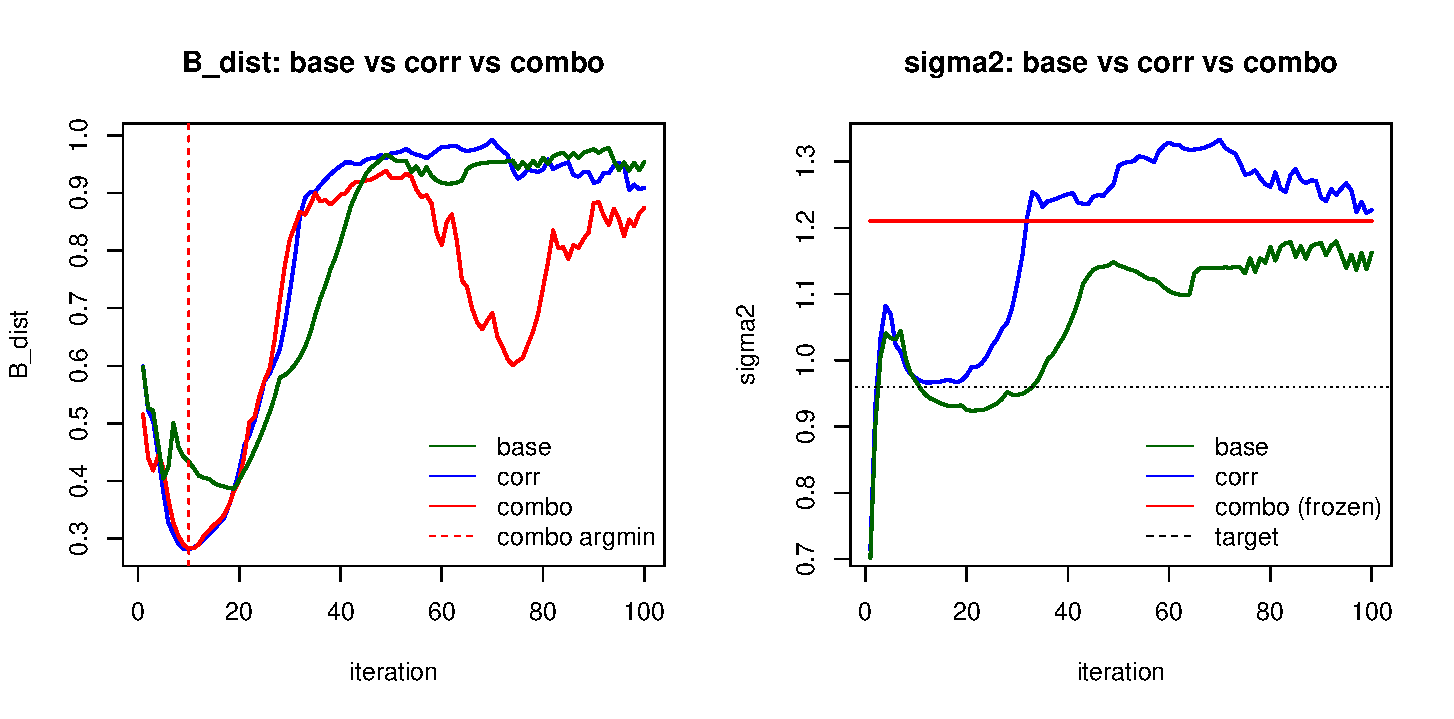
\includegraphics[width=0.95\textwidth]{figs/log-lik-unstable.pdf}
    \caption{Traces of the approximate log-likelihood, \texttt{B\_dist} and $\hat{\sigma}^{2}$ for the base, corrected $\bm{\lambda}$ and combo algorithms on simulated data ($Q=$\,, $J=$\,).}
    \label{fig:unstable-log-lik}
\end{figure}

The source of the failure is visible in the objective itself. Write $\hat{\bm{\lambda}}_{j}(\bm{\theta})$ for the mode of the group integrand $h_{j}(\cdot,\bm{\theta})$ and $\mathbf{H}_{j}(\bm{\lambda},\bm{\theta}):=-\nabla^{2}_{\bm{\lambda}}h_{j}(\bm{\lambda},\bm{\theta})$ for its curvature. The Laplace approximation to the marginal log-likelihood is
\begin{equation}
    \ell_{\text{LA}}(\bm{\theta})=\sum_{j=1}^{J}\left[h_{j}\big(\hat{\bm{\lambda}}_{j}(\bm{\theta}),\bm{\theta}\big)-\frac{1}{2}\log\Big|\mathbf{H}_{j}\big(\hat{\bm{\lambda}}_{j}(\bm{\theta}),\bm{\theta}\big)\Big|\right]-\frac{J}{2}\log|\bm{\Sigma}|,
    \label{eq:ellLA}
\end{equation}
with the details given in Appendix~\ref{app:mm-proofs}. A Laplace-EM M-step ascends only the $h$-part at the frozen mode. It treats the log-determinant as a constant. In our model the log-determinant is not a constant. It depends on $\bm{\theta}$ through two channels. The first channel is direct, since $\mathbf{H}_{j}$ contains $\bm{\theta}$. The second channel runs through the mode, since $\hat{\bm{\lambda}}_{j}(\bm{\theta})$ moves with $\bm{\theta}$. A $\bm{\theta}$-update can therefore raise the $h$-part while raising the curvature penalty by more. The approximate evidence then drops. This is exactly the pattern in Figure~\ref{fig:unstable-log-lik}.

% \citet{Yue2026} established majorize-minimize (MM) Laplace-EM algorithm to deal with this non-monotonicity. They used a surrogate function to replace simply Q-function. Given the current iterate estimated parameter $\bm{\Psi}^{(t)}$, they constructed a surrogate lower bound $Q_{\text{LA}}\left(\bm{\Psi} \mid \bm{\Psi}^{(t)}\right)$ for $\ell_{\text{LA}}\left(\bm{\Psi}\right)$ and maximize it over $\bm{\Psi}$, thereby increasing $\ell_{\text{LA}}\left(\bm{\Psi}\right)-\ell_{\text{LA}}\left(\bm{\Psi}^{(t)}\right)$. Concretely, $Q_{\text{LA}}$ is obtained by a Laplace expansion of the subject-level integral at the posterior mode $\hat{\bm{\lambda}}$ computed by the negative Hessian $\mathbf{H}$. 

\citet{Yue2026} met the same instability in a mixed-effects mixture-of-experts model with Gaussian responses and stabilized their Laplace-EM with a majorize-minimize (MM) strategy, combining a Jensen bound on the mixture term with a tangent-plane linearization of the log-determinant at the current curvature. Two features of their treatment matter here. First, their surrogate freezes the current mode inside the $h$-part, and the resulting ascent of $\ell_{\text{LA}}$ is asserted rather than derived from a minorization property. Second, the benchmark case in which no repair is needed at all is the single-expert Gaussian model. There the integrand is exactly quadratic in the random effect, the curvature does not depend on it, and the third-derivative tensor vanishes identically. Three consequences follow in that case. The Laplace approximation is exact. The mode channel in \eqref{eq:ellLA} is dead, because $\log|\mathbf{H}_{j}|$ cannot move when $\hat{\bm{\lambda}}_{j}(\bm{\theta})$ moves. And the log-determinant is a constant in the mean parameters, so maximizing $\ell_{\text{LA}}$ over that block reduces to maximizing $\sum_{j}h_{j}$. None of these facts survives once the integrand is not quadratic, which is the situation both for their expert mixture and for our multinomial responses. Our curvature depends on $\bm{\lambda}$ through the fitted probabilities, so both channels are alive. A direct transplant of a frozen-mode surrogate onto $\ell_{\text{LA}}$ therefore fails, and Proposition~\ref{prop:naive-obstruction} in Appendix~\ref{app:mm-proofs} makes the failure precise. The naive surrogate that freezes the mode and the curvature cannot be a tangent global minorizer of $\ell_{\text{LA}}$ at any iterate where the log-determinant has a nonzero gradient. The missing gradient is carried by $\partial_{\bm{\theta}}\mathbf{H}_{j}$ and by the contraction $\big\langle\mathbf{T}_{j},\hat{\mathbf{S}}_{j}\big\rangle$, and both vanish for the Gaussian mean parameters. The obstruction is first order, so it does not shrink near convergence. This is why the Gaussian construction cannot be inherited and a new monotone target is needed.


Following the general MM principle, we seek a surrogate $Q\big(\bm{\theta}\mid\bm{\theta}^{(t)}\big)$ with two properties for a suitable objective $F$. Property (P1) is global minorization, $Q\big(\bm{\theta}\mid\bm{\theta}^{(t)}\big)\leq F(\bm{\theta})$ for all $\bm{\theta}$. Property (P2) is tangency, $Q\big(\bm{\theta}^{(t)}\mid\bm{\theta}^{(t)}\big)=F\big(\bm{\theta}^{(t)}\big)$. Together they give the ascent chain
\begin{equation}
    F\big(\bm{\theta}^{(t+1)}\big)\geq Q\big(\bm{\theta}^{(t+1)}\mid\bm{\theta}^{(t)}\big)\geq Q\big(\bm{\theta}^{(t)}\mid\bm{\theta}^{(t)}\big)=F\big(\bm{\theta}^{(t)}\big),
    \label{eq:mm-ascent-chain}
\end{equation}
which is valid whenever the update does not decrease the surrogate. Exact maximization of $Q$ is never required. The whole difficulty is the choice of $F$. Proposition~\ref{prop:naive-obstruction} rules out $F=\ell_{\text{LA}}$ for the transplanted surrogate. We therefore change the objective instead of the inequality.
 
The repair promotes the modes to free coordinates. Define the group objective with a free expansion point $\bm{\lambda}$,
\begin{equation}
    \Phi_{j}(\bm{\theta},\bm{\lambda}):=h_{j}(\bm{\lambda},\bm{\theta})-\frac{1}{2}\log\big|\mathbf{H}_{j}(\bm{\lambda},\bm{\theta})\big|,
    \label{eq:Phi-def}
\end{equation}
and for $\bm{\Lambda}=(\bm{\lambda}_{1},\dots,\bm{\lambda}_{J})$ define the joint objective
\begin{equation}
    G(\bm{\theta},\bm{\Lambda}):=\sum_{j=1}^{J}\Phi_{j}(\bm{\theta},\bm{\lambda}_{j})-\frac{J}{2}\log|\bm{\Sigma}|.
    \label{eq:G-def}
\end{equation}
$G$ is an explicit smooth function of all its arguments. No implicit function $\hat{\bm{\lambda}}_{j}(\bm{\theta})$ appears in it. Two identities anchor $G$ to \eqref{eq:ellLA}, and both are proved as Lemma~\ref{lem:G-anchors}. First, $G\big(\bm{\theta},\hat{\bm{\Lambda}}(\bm{\theta})\big)=\ell_{\text{LA}}(\bm{\theta})$, so the profile of $G$ at the $h$-modes is exactly the Laplace evidence. Second, $\max_{\bm{\Lambda}}G(\bm{\theta},\bm{\Lambda})\geq\ell_{\text{LA}}(\bm{\theta})$, so the sup-profile dominates the Laplace evidence. The maximizing coordinate is the curvature-penalized mode $\bar{\bm{\lambda}}_{j}=\arg\max_{\bm{\lambda}}\Phi_{j}(\bm{\theta},\bm{\lambda})$ rather than the $h$-mode. Our algorithm ascends $G$ blockwise, in $\bm{\theta}$ with $\bm{\Lambda}$ frozen and in $\bm{\Lambda}$ with $\bm{\theta}$ frozen.
 
The $\bm{\theta}$-block needs a surrogate, because $\log\big|\mathbf{H}_{j}(\bm{\lambda}_{j}^{(t)},\bm{\theta})\big|$ is still a complicated function of $\bm{\theta}$. Only one inequality is used. The log-determinant is concave on positive definite matrices, so it lies below its tangent plane at the current curvature $\mathbf{H}_{j}^{(t)}:=\mathbf{H}_{j}\big(\bm{\lambda}_{j}^{(t)},\bm{\theta}^{(t)}\big)$. With $\mathbf{S}_{j}^{(t)}:=\big(\mathbf{H}_{j}^{(t)}\big)^{-1}$, this reads
\begin{equation}
    -\log|\mathbf{A}|\geq-\log\big|\mathbf{H}_{j}^{(t)}\big|-\operatorname{tr}\Big(\mathbf{S}_{j}^{(t)}\big(\mathbf{A}-\mathbf{H}_{j}^{(t)}\big)\Big)
    \label{eq:logdet-tangent}
\end{equation}
for every positive definite $\mathbf{A}$, with equality if and only if $\mathbf{A}=\mathbf{H}_{j}^{(t)}$ (Lemma~\ref{lem:logdet-tangent}). The base point of the tangent plane must be the current iterate. This choice makes the bound linear in the unknown curvature and exact at $\bm{\theta}^{(t)}$. Applying \eqref{eq:logdet-tangent} with $\mathbf{A}=\mathbf{H}_{j}\big(\bm{\lambda}_{j}^{(t)},\bm{\theta}\big)=-\nabla^{2}_{\bm{\lambda}}h_{j}\big(\bm{\lambda}_{j}^{(t)},\bm{\theta}\big)$ gives the surrogate
\begin{equation}
    Q\big(\bm{\theta}\mid\bm{\theta}^{(t)},\bm{\Lambda}^{(t)}\big):=\sum_{j=1}^{J}\left[h_{j}\big(\bm{\lambda}_{j}^{(t)},\bm{\theta}\big)-\frac{1}{2}\log\big|\mathbf{H}_{j}^{(t)}\big|-\frac{1}{2}\operatorname{tr}\Big(\mathbf{S}_{j}^{(t)}\big(-\nabla^{2}_{\bm{\lambda}}h_{j}(\bm{\lambda}_{j}^{(t)},\bm{\theta})-\mathbf{H}_{j}^{(t)}\big)\Big)\right]-\frac{J}{2}\log|\bm{\Sigma}|.
    \label{eq:Q-def}
\end{equation}
The tangency structure is now transparent. The $h$-terms and the $\log|\bm{\Sigma}|$ term are exact functions of $\bm{\theta}$, so no inequality touches them. The only inequality is \eqref{eq:logdet-tangent}, which is global in $\bm{\theta}$ and exact at $\bm{\theta}=\bm{\theta}^{(t)}$, where the trace term vanishes. Hence $Q\big(\cdot\mid\bm{\theta}^{(t)},\bm{\Lambda}^{(t)}\big)$ satisfies (P1) and (P2) for $F(\bm{\theta})=G\big(\bm{\theta},\bm{\Lambda}^{(t)}\big)$ (Proposition~\ref{prop:Q-minorize}). The everywhere-tangent lower bound therefore refers to $G\big(\cdot,\bm{\Lambda}^{(t)}\big)$ and not to $\ell_{\text{LA}}$. This is the price of the construction. By Proposition~\ref{prop:naive-obstruction} the price is unavoidable at first order. $G$ is the quantity our algorithm can make monotone.
 
\begin{theorem}
Assume $\sigma^{2}>0$ at every iterate, so that $\mathbf{H}_{j}(\bm{\lambda},\bm{\theta})\succ0$ for all arguments by Lemma~\ref{lem:H-pd}. Generate iterates by repeating, for $t=0,1,2,\ldots$:
\begin{enumerate}
    \item[(A)] $\bm{\theta}$-block: choose any $\bm{\theta}^{(t+1)}$ with $Q\big(\bm{\theta}^{(t+1)}\mid\bm{\theta}^{(t)},\bm{\Lambda}^{(t)}\big)\geq Q\big(\bm{\theta}^{(t)}\mid\bm{\theta}^{(t)},\bm{\Lambda}^{(t)}\big)$;
    \item[(B)] $\bm{\Lambda}$-block: choose any $\bm{\Lambda}^{(t+1)}$ with $\Phi_{j}\big(\bm{\theta}^{(t+1)},\bm{\lambda}_{j}^{(t+1)}\big)\geq\Phi_{j}\big(\bm{\theta}^{(t+1)},\bm{\lambda}_{j}^{(t)}\big)$ for every $j=1,\dots,J$.
\end{enumerate}
Then $G\big(\bm{\theta}^{(t+1)},\bm{\Lambda}^{(t+1)}\big)\geq G\big(\bm{\theta}^{(t)},\bm{\Lambda}^{(t)}\big)$ for every $t$. The sequence $G^{(t)}$ is non-decreasing and converges whenever it is bounded above.
\label{thm:G-non-decreasing}
\end{theorem}
 
The proof is in Appendix~\ref{app:mm-proofs}. Two remarks connect Theorem~\ref{thm:G-non-decreasing} back to the likelihood. Neither block requires exact maximization, so inexact and backtracked updates are covered. If in addition each accepted $\bm{\lambda}_{j}^{(t+1)}$ dominates the fresh $h$-mode in $\Phi_{j}$, then $G^{(t+1)}\geq\ell_{\text{LA}}\big(\bm{\theta}^{(t+1)}\big)$, so the monotone quantity sits above the Laplace evidence at the iterates (Corollary~\ref{cor:G-dominates}). This extra condition is available for free when the $h$-mode is kept in the candidate list of the $\bm{\Lambda}$-block.
 
Condition (B) only asks each $\Phi_{j}(\bm{\theta},\cdot)$ to go up. By Lemma~\ref{lem:Phi-grad}, the gradient of $\Phi_{j}$ in $\bm{\lambda}$ is
\begin{equation}
    \nabla_{\bm{\lambda}}\Phi_{j}(\bm{\theta},\bm{\lambda})=\nabla_{\bm{\lambda}}h_{j}(\bm{\lambda},\bm{\theta})-\frac{1}{2}\big\langle\mathbf{T}_{j}(\bm{\lambda},\bm{\theta}),\mathbf{H}_{j}^{-1}(\bm{\lambda},\bm{\theta})\big\rangle,
    \label{eq:Phi-grad}
\end{equation}
where $\mathbf{T}_{j}$ is the third-derivative tensor of $h_{j}$ and $\langle\cdot,\cdot\rangle$ is the contraction defined in \eqref{eq:T-contraction}. The curvature-penalized mode $\bar{\bm{\lambda}}_{j}$ solves $\nabla_{\bm{\lambda}}\Phi_{j}=\bm{0}$. The $h$-mode $\hat{\bm{\lambda}}_{j}$ solves the same equation with the second term dropped. The natural update for condition (B) is one Newton step for $\Phi_{j}$ started at the cheap point $\hat{\bm{\lambda}}_{j}$.
 
\begin{proposition}
Fix $\bm{\theta}$ and start at the $h$-mode $\hat{\bm{\lambda}}_{j}$. Approximate the Hessian of $\Phi_{j}$ by $\nabla^{2}_{\bm{\lambda}}\Phi_{j}\approx\nabla^{2}_{\bm{\lambda}}h_{j}=-\mathbf{H}_{j}$, which drops only the curvature of the penalty term. Then the Newton step for maximizing $\Phi_{j}$ is
\begin{equation}
    \bm{\lambda}^{\mathrm{new}}=\hat{\bm{\lambda}}_{j}-\frac{1}{2}\hat{\mathbf{S}}_{j}\big\langle\mathbf{T}_{j},\hat{\mathbf{S}}_{j}\big\rangle=\hat{\bm{\lambda}}_{j}+\bm{\mu}_{1,j},
    \label{eq:newton-step}
\end{equation}
where $\bm{\mu}_{1,j}=-\frac{1}{2}\hat{\mathbf{S}}_{j}\big\langle\mathbf{T}_{j},\hat{\mathbf{S}}_{j}\big\rangle$ is the Edgeworth mean correction of \eqref{eq: edgeworth}.
\label{prop:newton-edgeworth}
\end{proposition}
 
The proof is in Appendix~\ref{app:mm-proofs}. The same first-order object is reached by two independent routes. One route is the Edgeworth expansion of the posterior mean around the Laplace mode. The other route is the stationarity condition of the MM $\bm{\Lambda}$-block. Three consequences follow.
\begin{enumerate}
    \item The corrected E-step that we already tested is, to leading order, exactly the E-step the monotone algorithm needs. This explains why lambda correction term improves the estimation of $\mathbf{B}$ so consistently.
    \item It also explains why the correction alone does not restore monotonicity. The corrected algorithm still misses three things. (i) It drops the curvature-feedback term in the $\bm{\theta}$-update, i.e. the trace term of \eqref{eq:Q-def}. (ii) It evaluates the covariance $\hat{\mathbf{S}}_{j}$ at the $h$-mode instead of the exact curvature $\bar{\mathbf{S}}_{j}$ at the accepted $\bm{\lambda}_{j}$. (iii) It never checks that $\Phi_{j}$ actually went up.
    \item Point (iii) is cheap to fix. Evaluate $\Phi_{j}$ at $\hat{\bm{\lambda}}_{j}+c\,\bm{\mu}_{1,j}$ for $c\in\{1,\tfrac{1}{2},\tfrac{1}{4},\cdots\}$, fall back to $c=0$, and finally keep $\bm{\lambda}_{j}^{(t)}$ unchanged. Condition (B) then always holds, because the last fallback is always available. One evaluation of $\Phi_{j}$ costs one multinomial log-likelihood, one quadratic form, and one Cholesky log-determinant. Choosing the best candidate from this list, rather than the first acceptable one, additionally activates Corollary~\ref{cor:G-dominates}.
\end{enumerate}
 
Figure~\ref{fig:G-stable} reports the test on simulated data. The monitored quantity $G$ is non-decreasing along the whole run and converges before the iteration cap, as Theorem~\ref{thm:G-non-decreasing} guarantees. The comparison with the likelihood-criterion runs is honest rather than uniformly favorable. The minimal \texttt{B\_dist} reached under the likelihood criterion is slightly lower than the value returned under the $G$-criterion, so stopping on $G$ carries a small bias for $\mathbf{B}$. Moreover, \texttt{B\_dist} itself is not monotone even while $G$ is non-decreasing. Monotonicity of the objective therefore stabilizes the run, but it does not by itself locate the best $\mathbf{B}$ along the trajectory. This remains a real difficulty for estimation on real data, where \texttt{B\_dist} cannot be observed.
 
\begin{figure}[H]
    \centering
    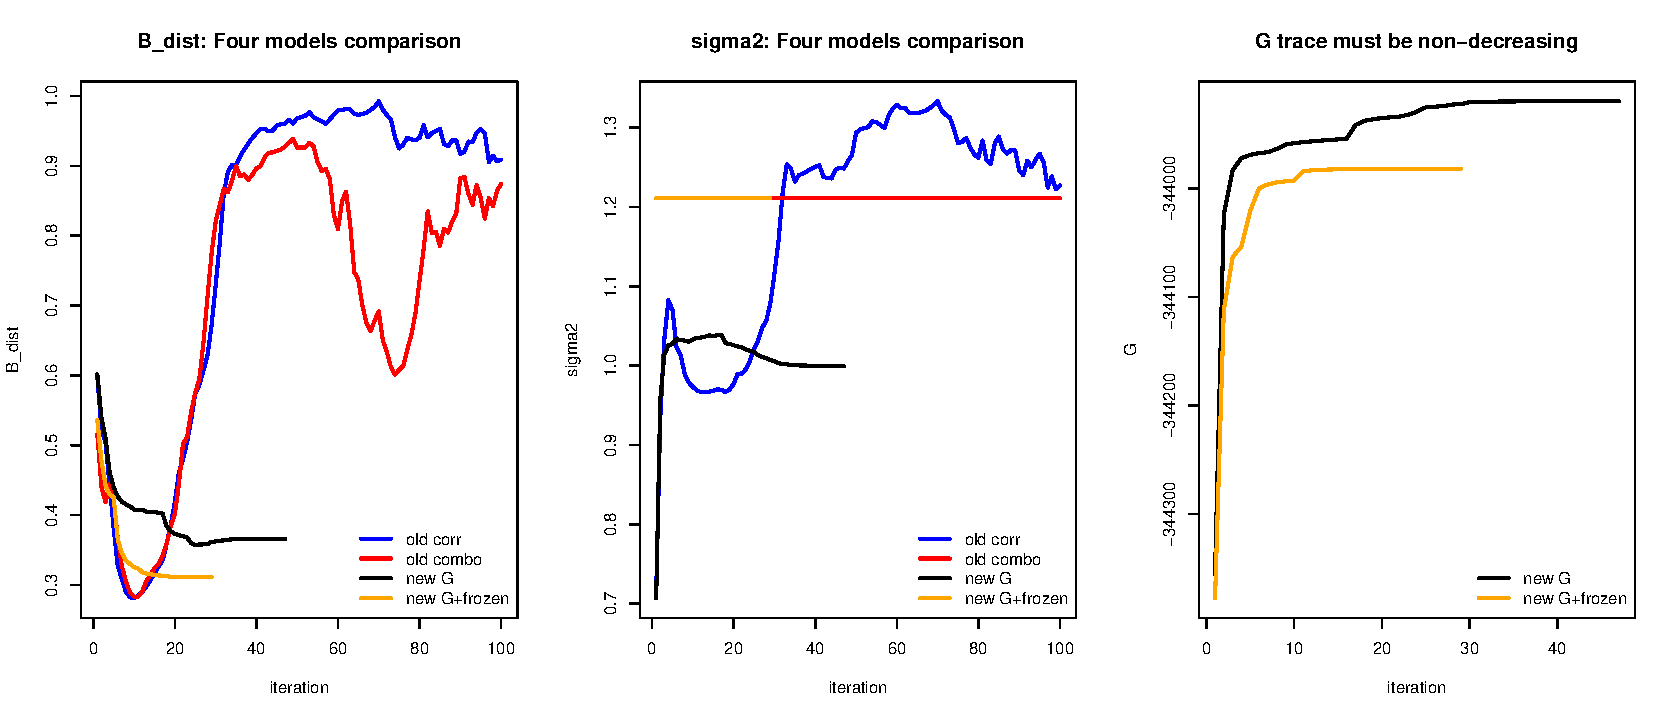
\includegraphics[width=0.99\textwidth]{figs/G-crition.pdf}
    \caption{Parameter estimation under the $G$-ascent algorithm compared with the likelihood convergence criterion.}
    \label{fig:G-stable}
\end{figure}

\section{Asymptotical Properties}
\label{sec:asymptotical-properties}

\iffalse
\subsection{Consistency and Asymptotic Normality of the Computable Estimators}
\label{subsec:la-g-asymptotics}

The exact-likelihood theory of Sections~\ref{sec:step0-identification}--\ref{sec:step2-normality} concerns the marginal maximum likelihood estimator. The algorithms of this thesis never touch the exact criterion. Laplace-EM targets $\ell_{\text{LA}}$ of \eqref{eq:ellLA}, and the monotone algorithm of Section~\ref{subsec:non-monotonicity} ascends $G$, whose profile over the free modes is $\ell_{G}(\bm{\theta}):=\max_{\bm{\Lambda}}G(\bm{\theta},\bm{\Lambda})$, with $\ell_{G}\geq\ell_{\text{LA}}$ by Lemma~\ref{lem:G-anchors}. Write $\ell_{J}(\bm{\theta}):=\sum_{j=1}^{J}\log L_{j}(\bm{\theta})$ for the exact marginal log-likelihood. This subsection establishes consistency and asymptotic normality for the maximizers of both computable criteria,
\begin{equation}
    \hat{\bm{\theta}}_{\text{LA}}:=\arg\max_{\bm{\theta}\in\Theta}\ell_{\text{LA}}(\bm{\theta}),\qquad\hat{\bm{\theta}}_{G}:=\arg\max_{\bm{\theta}\in\Theta}\ell_{G}(\bm{\theta}),
    \label{eq:computable-estimators}
\end{equation}
with ties broken by any measurable selection, and shows that the two estimators are asymptotically equivalent. The proof scheme follows \citet{Yue2026}: a uniform law of large numbers, a well-separated-maximum argument, and a score expansion under linear information growth for the per-group curvature. The structural difference from their treatment is stated in the comparison paragraph below.

Two error terms organize the whole analysis. Define $E_{\text{LA}}(\bm{\theta}):=\ell_{\text{LA}}(\bm{\theta})-\ell_{J}(\bm{\theta})$ and $E_{G}(\bm{\theta}):=\ell_{G}(\bm{\theta})-\ell_{\text{LA}}(\bm{\theta})$, so that each computable criterion equals the exact likelihood plus a correction. Write $N_{j}:=\sum_{i\in I_{j}}y_{ij\cdot}$ for the total count of group $j$ and $N:=\min_{j}N_{j}$. We work under the following conditions.
\begin{enumerate}
    \item[(D1)] Sampling and regime. Groups are independent, $J\to\infty$, and $Q$ and $K$ are fixed. The per-observation totals satisfy $y_{ij\cdot}\leq\bar{m}$ and all covariates lie in a fixed compact set. The group totals satisfy $N\to\infty$ and $\max_{j}N_{j}\leq\kappa\min_{j}N_{j}$ for a fixed $\kappa<\infty$.
    \item[(D2)] Parameter space. $\Theta$ is compact, $\bm{\theta}^{*}$ is interior, $\sigma^{2}\geq\sigma^{2}_{\min}>0$ on $\Theta$, and $\mathbf{B}$ obeys the PLT normalization of Section~\ref{sec:identifiability}.
    \item[(D3)] Exact-likelihood package. (i) $\sup_{\Theta}|J^{-1}\ell_{J}-\bar{\ell}|\xrightarrow{p}0$; (ii) $\bar{\ell}$ is continuous with a unique, well-separated maximum at $\bm{\theta}^{*}$; (iii) $J^{-1/2}\nabla\ell_{J}(\bm{\theta}^{*})\xrightarrow{d}\mathcal{N}(\bm{0},\bar{\mathbf{I}}(\bm{\theta}^{*}))$ with $\bar{\mathbf{I}}(\bm{\theta}^{*})\succ0$; (iv) $-J^{-1}\nabla^{2}\ell_{J}(\bm{\theta}_{J})\xrightarrow{p}\bar{\mathbf{I}}(\bm{\theta}^{*})$ along every sequence $\bm{\theta}_{J}\xrightarrow{p}\bm{\theta}^{*}$. These are exactly the uniform concentration, identification, score CLT and Hessian convergence results of Sections~\ref{sec:step1-concentration}, \ref{sec:step0-identification} and \ref{sec:step2-normality}, and they enter only as inputs.
    \item[(D4)] Information growth. There are $c_{0},r_{0}>0$ with $\mathbf{H}_{j}(\bm{\lambda},\bm{\theta})\succeq c_{0}N_{j}\mathbf{I}_{Q}$ whenever $\|\bm{\lambda}-\hat{\bm{\lambda}}_{j}(\bm{\theta})\|\leq r_{0}$, for every $\bm{\theta}\in\Theta$ and every $j$. This is the analogue of condition (B3) of \citet{Yue2026}, and it strengthens the global floor $\mathbf{H}_{j}\succeq\bm{\Sigma}^{-1}$ of Lemma~\ref{lem:H-pd} on a ball around the mode.
    \item[(D5)] Error derivatives. On a fixed neighborhood of $\bm{\theta}^{*}$, $\|\nabla E_{\text{LA}}\|\leq CJ/N$, $\|\nabla^{2}E_{\text{LA}}\|\leq CJ/N$ and $\|\nabla^{2}E_{G}\|\leq CJ/N$. The value-level analogues and the bound on $\nabla E_{G}$ are proved in Proposition~\ref{prop:criteria-gap} below; (D5) is the remaining derivative-level control, in the spirit of the approximate-likelihood framework of \citet{Ogden2017}, and its leading term is the object expanded in Section~\ref{sec:gap-one}.
\end{enumerate}

The first result quantifies how far the computable criteria sit from the exact likelihood. The per-group derivative-scale bounds it uses are automatic for multinomial responses and are recorded as Lemma~\ref{lem:tensor-scale}, the analogue of condition (B4) of \citet{Yue2026}.

\begin{proposition}
Assume (D1), (D2) and (D4). There are $N_{0}$ and $C$, depending only on $Q$, $K$, $\Theta$, the design bounds and $(c_{0},r_{0})$, such that for every $\bm{\theta}\in\Theta$ and every $j$ with $N_{j}\geq N_{0}$ the following hold. First, $\ell_{J}(\bm{\theta})=\ell_{\text{LA}}(\bm{\theta})+\sum_{j=1}^{J}\log Z_{j}(\bm{\theta})$, where $Z_{j}(\bm{\theta})$ is the group-$j$ normalizing ratio of \eqref{eq:posterior-tilt}, and $|\log Z_{j}(\bm{\theta})|\leq C/N_{j}$. Second, the curvature-penalized mode $\bar{\bm{\lambda}}_{j}(\bm{\theta})$ is unique and satisfies $\|\bar{\bm{\lambda}}_{j}-\hat{\bm{\lambda}}_{j}\|\leq C/N_{j}$ and $\bar{\bm{\lambda}}_{j}=\hat{\bm{\lambda}}_{j}+\bm{\mu}_{1,j}+O(N_{j}^{-2})$, and $0\leq E_{G}(\bm{\theta})\leq C\sum_{j}N_{j}^{-1}$. Third, $\|\nabla E_{G}(\bm{\theta})\|\leq C\sum_{j}N_{j}^{-1}$. In particular $\sup_{\Theta}|\ell_{A}-\ell_{J}|\leq C\kappa J/N$ for $A\in\{\text{LA},G\}$.
\label{prop:criteria-gap}
\end{proposition}

The proof is in Appendix~\ref{app:asymptotics-proofs}. The reading is simple. Both criteria differ from the exact likelihood by $O(J/N)$ in value, the $G$-versus-LA gap is one-sided and of the same order, and the leading terms of the two scores cancel exactly, through the same object $\bm{\mu}_{1,j}$ that defines the Edgeworth correction. Everything the algorithms optimize is therefore an $O(J/N)$ perturbation of $\ell_{J}$, and the two theorems below are transfer theorems.

\begin{theorem}
Assume (D1)--(D4). Then $\hat{\bm{\theta}}_{\text{LA}}\xrightarrow{p}\bm{\theta}^{*}$ and $\hat{\bm{\theta}}_{G}\xrightarrow{p}\bm{\theta}^{*}$ as $J\to\infty$.
\label{thm:computable-consistency}
\end{theorem}

The argument transports the uniform concentration of (D3)(i) to both computable criteria through Proposition~\ref{prop:criteria-gap} and then applies the well-separation step, exactly as in Propositions~1 and~2 of \citet{Yue2026}; their envelope construction is not needed here, because uniform concentration of the exact likelihood is already available.

\begin{theorem}
Assume (D1)--(D5) and $\sqrt{J}/N\to0$. Then, for $A\in\{\text{LA},G\}$,
\begin{equation}
    \sqrt{J}\big(\hat{\bm{\theta}}_{A}-\bm{\theta}^{*}\big)\xrightarrow{d}\mathcal{N}\big(\bm{0},\bar{\mathbf{I}}(\bm{\theta}^{*})^{-1}\big),\qquad\sqrt{J}\big(\hat{\bm{\theta}}_{G}-\hat{\bm{\theta}}_{\text{LA}}\big)\xrightarrow{p}\bm{0}.
    \label{eq:computable-an}
\end{equation}
\label{thm:computable-an}
\end{theorem}

Both estimators attain the same first-order limit as the exact maximum likelihood estimator, with the exact-likelihood information in the variance. The rate condition weighs the two error sources against each other. The stochastic error is $O_{p}(J^{-1/2})$ and the approximation bias is $O(N^{-1})$, so $\sqrt{J}/N\to0$ is exactly the regime in which the bias is negligible at the CLT scale; this is the classical condition of \citet{Vonesh1996} for Laplace-based estimation. The second display says that certifying monotonicity through $G$ costs nothing asymptotically. The certificate objective sits above $\ell_{\text{LA}}$ by $O(J/N)$, its score gap is $O(J/N)$ after the exact cancellation of Lemma~\ref{lem:G-score-cancel}, and the two estimators are interchangeable to first order.

Two comparisons with \citet{Yue2026} locate the contribution. First, their consistency theorem holds at fixed cluster sizes because their condition (A4) assumes that the population Laplace criterion is maximized at the true parameter, which absorbs the entire approximation bias into an assumption. Our Proposition~\ref{prop:criteria-gap} replaces that assumption by a proved $O(1/N)$ bound, and consistency to the truth then genuinely requires $N\to\infty$. This is the honest form of the statement for multinomial responses, where the Laplace error is nonzero at every sample size. Second, their asymptotic normality result is a sandwich-form CLT for the regression block around the maximizer of the population Laplace criterion. The fixed-$N$ analogue holds here as well: without the rate condition, $\hat{\bm{\theta}}_{A}$ is asymptotically normal around a pseudo-true value $\bm{\theta}^{*}_{A}$ with sandwich variance, and Lemma~\ref{lem:pseudo-true} bounds $\|\bm{\theta}^{*}_{A}-\bm{\theta}^{*}\|\leq C/N$ (Remark~\ref{rem:sandwich}). Their conditions (B3) and (B4) reappear here as (D4) and Lemma~\ref{lem:tensor-scale}, and their Lemma~1, which localizes the Laplace mode around the true random effect, is replaced by Lemma~\ref{lem:mode-localization}, which localizes the curvature-penalized mode around the Laplace mode; that is the additional step the $G$ criterion needs.

Two remarks on scope. The leading term of $\log Z_{j}$ is an explicit contraction of third and fourth derivatives \citep{ShunMcCullagh1995}, and the corrected E-step of Section~\ref{subsec:corrected-lambda} targets exactly the mean-level part of this object; a formal bias-reduction theorem for the corrected estimator is left open. All constants in this subsection depend on the fixed dimension $Q$; the joint growth regime, in which $Q$ increases with $J$, is the subject of Section~\ref{sec:joint-growth} and is conjectured there to require $J\gg Q^{c}\log Q$.
\fi
\iffalse
In this section, we adopt the processes established by \citet{Cui2026} and write the proof of analytic results based on the converged estimation $\hat{\bm{\theta}}_{n}:=\arg\max_{\bm{\theta}}\sum_{j}\ell_{\text{obs}}(\bm{\theta}, \bm{y}_{j})$, where $\ell_{\text{obs}}(\bm{\theta}, \bm{y}_{j}):=\log p(\bm{y}_{j}, \bm{\theta})$ denotes the marginal log-likelihood of group $j$.

\subsection{Consistency}

Let $\bar{\ell}(\bm{\theta}):=\mathbb{E}_{\theta^{*}}[\ell_{\text{obs}}(\bm{\theta},\bm{y})]$ and $\bar{I}(\bm{\theta}^{*}):=-\nabla^{2}\bar{\ell}(\bm{\theta}^{*})$ denote the population Fisher information. According to the Wald consistency process, there are three steps for the proof of consistency.

\subsubsection{Identification}

\begin{lemma}
    For any $\bm{\theta}$, $\bar{\ell}(\bm{\theta})\leq \bar{\ell(\bm{\theta^{*}})}$ with equality if and only if the ratio $\dfrac{p(\bm{y},\bm{\theta})}{p(\bm{y},\bm{\theta}^{*})}$ is a.s  constant.
    \label{lem:identification1}
\end{lemma}

\begin{proof}
    For any $\bm{\theta}$, we apply Jensen's inequality to the strictly convex function,
    \begin{align*}
        \bar{\ell}(\bm{\theta})-\bar{\ell}(\bm{\theta}^{*})&=\mathbb{E}_{\bm{\theta}^{*}}\left[\log \dfrac{p(\bm{y},\bm{\theta})}{p(\bm{y},\bm{\theta}^{*})}\right]\\
        &\leq \log \mathbb{E}_{\bm{\theta}^{*}}\left[ \dfrac{p(\bm{y},\bm{\theta})}{p(\bm{y},\bm{\theta}^{*})}\right]\\
        &=\log \int \dfrac{p(\bm{y},\bm{\theta})}{p(\bm{y},\bm{\theta}^{*})}p(\bm{y},\bm{\theta}^{*})\,d\bm{y}=\log \int p(\bm{y},\bm{\theta})\,d\bm{y}=0.
    \end{align*}
\end{proof}

In simple case with regularity conditions, the function $\theta \mapsto P^{\theta}_{y}$ is an injection in Lemma~\ref{lem:identification1}, establishing consistency of $\bm{\theta}$. However, our FA-DMR model suffers from rotational and signed indeterminacy, thus consistency cannot be concluded here. Instead of structuring the global injection, we use local curvature as the surrogate of global injection.

\begin{lemma}
    Suppose the twice differentiation for $\bar{\ell}$ holds, then $\nabla_{\bm{\theta}}\bar{\ell}(\bm{\theta}^{*})=0$ and $\nabla_{\bm{\theta}}^{\top}\nabla_{\bm{\theta}}\bar{\ell}(\bm{\theta}^{*})=-\bar{I}(\bm{\theta}^{*})$.
    \label{lem:identification2}
\end{lemma}

\begin{proof}
    With regularity conditions hold, we can exchange the calculation $\mathbb{E}_{\bm{\theta}^{*}}[\cdot]$ and $\nabla_{\bm{\theta}}(\cdot)$.
\end{proof}

\begin{theorem}[Local Identification]
    Suppose $\bar{\ell}$ is twice continuously differentiable in a neighborhood of $\bm{\theta}$, denoted $\Theta$ (the PLT-constrained parameter space) and $\bar{I}(\bm{\theta}^{*})\succ 0$. Then there is a neighborhood $U$ of $\bm{\theta}^{*}$ such that $\bm{\theta}^{*}$ is the unique maximizer of $\bar{\ell}$ in neighborhood $U$. That is, any $\bm{\theta}\in U\setminus \{\bm{\theta}^{*} \}$, either $\bar{\ell}(\bm{\theta})<\bar{\ell}(\bm{\theta}^{*})$ or no such $\bm{\theta}$ with $\bar{\ell}(\bm{\theta})=\bar{\ell}(\bm{\theta}^{*})$ exists in $U\setminus \{\bm{\theta}^{*}\}$ at all.
\end{theorem}

\begin{proof}
    By Lemma~\ref{lem:identification1}, $\bar{\ell}(\bm{\theta})\leq \bar{\ell(\bm{\theta^{*}})}$ everywhere, so it suffices to rule out a sequence $\bm{\theta}_{n}\to \bm{\theta}^{*}$, $\bm{\theta}_{n}\neq \bm{\theta}^{*}$, with $\bar{\ell}(\bm{\theta})= \bar{\ell(\bm{\theta^{*}})}$ for every $n$. Suppose toward a contradiction such a sequence exists. By Lemma~\ref{lem:identification2} and Taylor expansion with Peano error, we have,
    \begin{equation*}
        0=\bar{\ell}(\bm{\theta}_{n})-\bar{\ell}(\bm{\theta}^{*})=-\dfrac{\left(\bm{\theta}_{n}-\bm{\theta}^{*}\right)^{\top}\bar{I}(\bm{\theta}^{*})\left(\bm{\theta}_{n}-\bm{\theta}^{*}\right)}{2}+o\left(\|\bm{\theta}_{n}-\bm{\theta}^{*}\|^{2}\right)
    \end{equation*}
    Divided by $\|\bm{\theta}_{n}-\bm{\theta}^{*}\|^{2}>0$ and write the unit vector  $\bm{u}_{n}:=\left(\bm{\theta}_{n}-\bm{\theta}^{*}\right)/\|\bm{\theta}_{n}-\bm{\theta}^{*}\|$. Thus,
    \begin{equation*}
        0=-\dfrac{1}{2}\bm{u}_{n}^{\top}\bar{I}(\bm{\theta}^{*})\bm{u}_{n}+o(1).
    \end{equation*}
    Since $\{\bm{u}_{n}\}$ lies on the compact unit sphere, a subsequence converges to the unit vector $\bm{u}$ passing to the limit along that subsequence, thus $\bm{u}_{n}^{\top}\bar{I}(\bm{\theta}^{*})\bm{u}_{n}=0$. However, $\bar{I}(\bm{\theta}^{*})\succ 0$, which implies that $\bm{u}_{n}^{\top}\bar{I}(\bm{\theta}^{*})\bm{u}_{n}>0$ for any unit vector $\bm{u}$ and leads to a contradiction. Hence no such sequence exists. 
\end{proof}
\fi

\iffalse
\subsubsection{Uniform Convergence}

After proof of identification, the target is uniform convergence 
\begin{equation}
    \sup_{\bm{\theta}\in \Theta}|\ell_{n}\left(\bm{\theta}\right)-\bar{\ell}\left(\bm{\theta}\right)|\to 0,
\end{equation}
in probability by Lipschitz-envelope Glivenko-Cantelli method. We separate the work into two parts: the pointwise LLN and uniformly Lipschitz envelope.

\begin{lemma}
    For any $\bm{\theta}\in \Theta$ and any data point $\bm{y}$ in the finite support of a single group's data, we have $\ell_{\text{obs}}\left(\bm{\theta},\bm{y}\right)\in \left[L\left(\bm{y}\right), U\left(\bm{y}\right)\right]$ for finite, $\bm{\theta}$-independent bounds $L$ and $U$. Consequently, $\bar{\ell}(\bm{\theta})=\mathbb{E}_{\bm{\theta}^{*}}[\ell_{\text{obs}}(\bm{\theta},\bm{y})]$ is finite for any $\bm{\theta}$.
    \label{lem:uniconverge1}
\end{lemma}

\begin{proposition}[Pointwise LLN]
    For any fixed $\bm{\theta}$, $\ell_{n}\left(\bm{\theta}\right)\to \bar{\ell}\left(\bm{\theta}\right)$ almost surely as $J\to \infty$.
    \label{prop:uniconverge2}
\end{proposition}

\begin{proof}
    Since the group effect $\bm{\lambda}_{j}\sim \mathcal{N}\left(0,\bm{\Sigma}(\bm{\theta}^{*})\right)$ are independent and $\bm{y}_{j}\mid \bm{\lambda}_{j}$ conditionally independent of other groups, $\{\ell_{\text{obs}}\}_{j=1}^{J}$ are independent and identically distributed across group $j$. With finite mean $\bar{\ell}\left(\bm{\theta}\right)$ by Lemma~\ref{lem:uniconverge1}, we apply the strong law of large numbers directly, that is,
    \begin{equation*}
        \ell_{n}\left(\bm{\theta}\right)=\dfrac{1}{J}\sum_{j=1}^{J} \ell_{\text{obs}, j}\left(\bm{\theta}\right)\to \mathbb{E}_{\bm{\theta}^{*}}[\ell_{\text{obs}}(\bm{\theta})]=\bar{\ell}\left(\bm{\theta}\right),
    \end{equation*}
    almost surely.
\end{proof}

Proposition~\ref{prop:uniconverge2} requires both the regularity conditions and $J\to\infty$, which is not the same regime as we discussed before. Although our model has two levels and 3 indexes (I observations, J groups and Q categories), only group-level parameters determine the properties based on group effect $\bm{\lambda}_{j}$. We call this as sparse multinomial regime in some applications, for example, the forensic DNA profiling.

\begin{lemma}[Lipschitz Envelope]
    For any $\bm{\theta}$ and $\bm{\theta}^{'}$ in compact, convex and PLT-constrained space $\Theta$, we have,
    \begin{equation*}
        |\ell_{\text{obs}}\left(\bm{\theta},\bm{y}\right)-\ell_{\text{obs}}\left(\bm{\theta}^{'},\bm{y}\right)|\leq L(\bm{y}_{j})\|\bm{\theta}-\bm{\theta}^{'}\|,
    \end{equation*}
    where the Lipschitz constant is,
    \begin{equation*}
        L(\bm{y}_{j}):=\sup_{\bm{\theta}\in \Theta}\|\nabla_{\bm{\theta}}\ell_{\text{obs}}\left(\bm{\theta},\bm{y}_{j}\right)\|.
    \end{equation*}
    Using Lemma and the Cauthy-Schwarz bound,
    \begin{equation*}
        L(\bm{y}_{j})\leq \sup_{\bm{\theta}\in \Theta}\left\{c(\bm{\theta})\left(C_{Q}(\bm{\theta})\dfrac{Q}{m}+\|\hat{\bm{\lambda}}(\bm{\theta},\bm{y}_{j})\|^{2}\right)+c^{'}(\bm{\theta})\right\}
    \end{equation*}
    for continuous and $\Theta$-bounded functions $c$, $c^{'}$ of $\bm{\theta}$.
\end{lemma}

\begin{proposition}
    $\mathbb{E}_{\bm{\theta}^{*}}[L(\bm{y})]<\infty$.
\end{proposition}

\begin{theorem}
    For fixed $Q$,
    \begin{equation*}
        \sup_{\bm{\theta}\in \Theta}|\ell_{n}(\bm{\theta})-\bar{\ell}(\bm{\theta})|\to 0
    \end{equation*}
    in probability as $J\to \infty$.
    \label{thm:uniconverge}
\end{theorem}

Throughout, $\Theta\in U$ is a compact, convex neighborhood of $\bm{\theta}^{*}$ contained in the neighborhood $U$. 

\subsection{Asymptotic Normality}

\begin{lemma}
    For any $\epsilon>0$ with an nonempty set $K_{\epsilon}:=\left\{\bm{\theta}\in \Theta: \|\bm{\theta}-\bm{\theta}^{*}\|\geq \epsilon\right\}$, 
    \begin{equation*}
        \sup_{\bm{\theta}\in K_{\epsilon}}\bar{\ell}(\bm{\theta})<\bar{\ell}(\bm{\theta}^{*}).
    \end{equation*}
\end{lemma}

\begin{proof}
    As we defined, $K_{\epsilon}$ is a closed subset of the compact set $\Theta$, so $K_{\epsilon}$ is compact. The continuous function $\bar{\ell}$ achieves its maximum on $K_{\epsilon}$ at some $\bm{\theta}_{\epsilon}\in K_{\epsilon}$. Since $\|\bm{\theta}_{\epsilon}-\bm{\theta}^{*}\|\geq \epsilon>0$, $\bm{\theta}_{\epsilon}\neq \bm{\theta}^{*}$ and $\bm{\theta^{*}}$ being the unique maximizer of $\bar{\ell}$ on $K_{\epsilon}\subseteq \Theta$, we conclude that $\bar{\ell}(\bm{\theta}_{\epsilon})<\bar{\ell}(\bm{\theta}^{*})$ strictly.
\end{proof}

\begin{theorem}
    $\hat{\bm{\theta}}_{n}\to \bm{\theta}^{*}$ in probability as $J\to \infty$.
\end{theorem}

\begin{proof}
    For a fixed $\epsilon>0$, let $\delta=\bar{\ell}(\bm{\theta}^{*})-\sup_{\bm{\theta}\in K_{\epsilon}}\bar{\ell}(\bm{\theta})$. By Lemma~\ref{lem:identification1}, $\delta>0$. By Theorem~\ref{thm:uniconverge}, $\mathbb{P}\left(\sup_{\bm{\theta}\in \Theta}|\ell_{n}(\bm{\theta})-\bar{\ell}(\bm{\theta})|< \frac{\delta}{2}\right)=1$. Since $\hat{\bm{\theta}}_{n}$ maximizes $\ell_{n}$ over $\Theta$, where the true value $\bm{\theta}^{*}$ holds, thus,
    \begin{equation*}
        \ell_{n}(\hat{\bm{\theta}}_{n})\geq \ell_{n}(\bm{\theta}^{*})>\bar{\ell}(\bm{\theta}^{*})-\dfrac{\delta}{2},
    \end{equation*}
\end{proof}
\fi
\iffalse
\section{Complexity Analysis}
\label{sec:complexity-analysis}

\subsection*{Numerical Equivalence of Two Implementations}
\label{sec:equivalence}

Before quantifying the speed-up efficiency, we establish that it is not bought at the cost of accuracy.
The Woodbury implementation and the dense reference compute the same quantities because the
Woodbury identity being an exact algebraic equivalence rather than an approximation. We verify
this directly at the three points where the two implementations differ in arithmetic but must
agree in value.

\begin{table}[H]
\centering
\caption{Numerical equivalence of the dense and Woodbury implementations
($K=2$, single group). Errors are maximum absolute differences; the mode is
compared by both correlation and maximum absolute difference.}
\label{tab:equivalence}
\begin{tabular}{@{}rcccc@{}}
\toprule
$Q$ & $\bm\Sigma^{-1}v$ error & mode corr. & mode max.\ diff. & $\log|\widehat{\mathbf S}_j|$ error \\
\midrule
50   & $1.1e^{-14}$ & $1.0000$ & $5.3e^{-8}$ & $[X]$ \\
100  & $2.8e^{-14}$ & $1.0000$ & $4.6e^{-10}$ & $[X]$ \\
200  & $9.6e^{-14}$ & $1.0000$ & $3.6e^{-10}$ & $[X]$ \\
500  & $6.3e^{-14}$ & $1.0000$ & $5.0e^{-10}$ & $[X]$ \\
1000 & $2.6e^{-13}$ & $1.0000$ & $2.4e^{-8}$ & $[X]$ \\
\bottomrule
\end{tabular}
\end{table}

\subsection*{Numerical Gap of $\mathbf{S}$  and $\mathbf{S}^{P}$}
\label{sec:numerical gap}

The equivalence of Table~\ref{tab:Shat-compare} established that the two implementations agree on the posterior model. However, the mode is affected both by the output of E-step and Laplace curvature $\hat{\mathbf{S}}_{j}$. We have found in Proposition~\ref{prop:diff-s} and \eqref{eq:covariance-relation} that Poisson surrogate $\hat{\mathbf{S}}^{P}_{j}$ over-states the curvature and hence under-states the variance, which has been shown by the estimation of $\sigma^{2}$ in Table~\ref{tab:Shat-compare}. 

\begin{table}[H]
\centering
\caption{Full-EM comparison of the dense reference against the Woodbury fitter with the
exact and surrogate posterior curvatures ($Q=30$, $K=2$, $J=20$, $I_j=12$, $\sigma^2_{\text{true}}=0.30$).
The mode-based quantities are shared. The two Woodbury variants differ only in
$\hat{\mathbf{S}}_j$.}
\label{tab:Shat-compare}
\begin{tabular}{@{}cccc@{}}
\toprule
Quantity & Dense + $\mathbf S$ & Woodbury + $\mathbf S$ & Woodbury + $\mathbf S^{P}$ \\
\midrule
Final Laplace log-ev      & $-103349.10$ & $-103349.08$ & $-103379.49$ \\
$\hat{\sigma}^2$            & $0.2556$     & $0.2557$     & $0.2447$ \\
$d(\hat{\mathbf B},\mathbf B_{\text{true}})$ & $0.5019$ & $0.4956$ & $0.4743$ \\
$\lambda$ mode correlation      & $0.9514$     & $0.9515$     & $0.9515$ \\
log-ev non-decreasing     & Yes          & Yes          & Yes \\
\midrule
$|\log\text{-ev} - \text{dense}|$ & --- & $0.017$ & $30.39$ \\
$|\widehat\sigma^2 - \text{dense}|$ & --- & $0.0001$ & $0.0109$ \\
\bottomrule
\end{tabular}
\end{table}

\subsection*{Acceleration Efficiency}
\label{sec:acceleration-efficiency}

Across all $Q$, the prior-precision action and the analytic log-determinant agree with the
dense computations to $[X]$ (order $10^{-14}$, i.e.\ floating-point round-off), and the two
posterior modes coincide with correlation $[X]$ and maximum absolute difference $[X]$
(order $10^{-8}$, the tolerance of the shared gradient stopping rule). The two implementations
are thus numerically indistinguishable, and the timing comparisons that follow contrast two
exact routes to identical estimates, differing only in computational cost.

\begin{table}[H]
\centering
\caption{Per-operation asymptotic complexity: dense base vs.\ Woodbury.
$Q$ categories, $K$ factors ($K\ll Q$), $I_j$ within-group observations, $P$ covariates.}
\label{tab:complexity-asymptotic}
\begin{tabular}{@{}cccc@{}}
\toprule
Operation (per group / per inner iteration) & Dense & Woodbury & Speed-up \\
\midrule
E-step Newton direction $(-\mathbf H)^{-1}\mathbf g$      & $O(Q^3)$   & $O(QK^2+K^3)$ & $O(Q^2/K^2)$ \\
Gradient / softmax / line-search $\ell$                   & $O(I_jQ)$  & $O(I_jQ)$     & $1$ \\
Posterior curvature $\widehat{\mathbf S}_j$              & $O(Q^3)$   & $O(QK^2)$     & $O(Q^2/K^2)$ \\
$\log|\widehat{\mathbf S}_j|$                            & $O(Q^3)$   & $O(QK^2+K^3)$ & $O(Q^2/K^2)$ \\
Rubin-Thayer $\mathbf B$ update (per RT iter)           & $O(Q^3)$   & $O(Q^2K)$     & $O(Q/K)$ \\
$\log|\bm\Sigma|$                                        & $O(Q^3)$   & $O(K^3)$      & $O(Q^3/K^3)$ \\
Fixed-effect $\mu,\bm\phi$ ($Q$ Poisson GLMs)            & $O(Q\,g(I_j,P))$ & $O(Q\,g(I_j,P))$ & $1$ \\
\bottomrule
\end{tabular}
\end{table}

Table~\ref{tab:complexity-asymptotic} isolates the source of the speed-up. Every operation
whose dense cost is $O(Q^3)$ becomes $O(QK^2)$ or $O(Q^2K)$ under the Woodbury
factorisation, while the two operations that are \emph{not} functions of the
diagonal-plus-low-rank structure---the $O(I_jQ)$ objective/softmax evaluations and the $Q$
independent Poisson GLMs of the fixed-effect step---are, correctly, left unchanged. The
acceleration is therefore confined to exactly the linear-algebra that the PME-induced
structure makes reducible, and to nothing else; this is why the
per-operation speed-up columns scale as $Q^2/K^2$ for the E-step and $Q/K$ for the
Rubin--Thayer update, and not as a single global constant.
\fi
\iffalse
\begin{table}[H]
\centering
\caption{Measured single-solve wall-time (this machine, $K=2$). Dense forms and
solves the $Q\times Q$ system; Woodbury uses the diagonal-plus-rank-$K$ factorisation.
[Fill in from your own runs.]}
\label{tab:solve-timing}
\begin{tabular}{@{}rccccc@{}}
\toprule
$Q$ & Dense (ms) & Woodbury (ms) & Speed-up & $\ell(\cdot)$ eval (ms) & Peak mem \\
\midrule
50   & \phantom{000.00} & \phantom{00.00} & \phantom{000}$\times$ & \phantom{0.00} & \\
100  &  &  & $\times$ &  & \\
200  &  &  & $\times$ &  & \\
500  &  &  & $\times$ &  & \\
1000 &  &  & $\times$ &  & \\
\bottomrule
\end{tabular}
\end{table}

The measured per-solve speed-up grows with $Q$, from $[X]\times$ at $Q=50$ to $[X]\times$ at
$Q=1000$, consistent with the $O(Q^2/K^2)$ prediction of
Table~\ref{tab:complexity-asymptotic}: at fixed $K$, doubling $Q$ should roughly quadruple the
ratio, and the measured column follows this trend to within the constant factors of an
interpreted runtime. The final column records the cost of a single evaluation of the
true log-posterior $\ell$, which the backtracking line search calls one to a few times per
Newton step in \emph{both} methods. Because this evaluation is $O(I_jQ)$ and is not reducible
by the factorisation, it sets a floor on per-step cost once the Woodbury solve has collapsed
to sub-millisecond; at large $Q$ it becomes the dominant per-step term, and the full
$O(Q^3)\!\to\!O(QK^2)$ gain in the solve is only partially visible in an interpreted
implementation. We report it explicitly rather than absorb it, because it explains the gap
between the solve-level and end-to-end speed-ups discussed next.

\begin{table}[H]
\centering
\caption{End-to-end per-EM-iteration wall-time on simulated data
($J=\;$[\,], $I_j=\;$[\,], $K=2$). Reports the full E-step + M-step cost including
the $O(I_jQ)$ objective evaluations. [Fill in from your own runs.]}
\label{tab:endtoend-timing}
\begin{tabular}{@{}rcccc@{}}
\toprule
$Q$ & Dense (s) & Woodbury (s) & Speed-up & Notes \\
\midrule
30   &  &  & $\times$ & (small $Q$: Woodbury overhead may dominate) \\
100  &  &  & $\times$ & \\
400  &  &  & $\times$ & \\
1000 &  &  & $\times$ & \\
\bottomrule
\end{tabular}
\end{table}

At the level of a full EM iteration the speed-up is smaller than the single-solve figure---
$[X]\times$ versus $[X]\times$ at $Q=[X]$---and this gap is expected, not anomalous: an EM
iteration spends time in the $O(I_jQ)$ objective evaluations and the $Q$ Poisson GLMs, neither
of which the factorisation touches, so by Amdahl's law the achievable end-to-end gain is
bounded by the fraction of runtime that is reducible linear algebra. The effect is most
visible at small $Q$: at $Q=[X]$ the Woodbury fitter is in fact \emph{slower} than the dense
one, because the reducible $Q^3$ term has not yet grown large enough to offset the fixed
overhead of forming the $K\times K$ factors and the surrogate direction, which the dense
method does not incur. The two methods cross over near $Q\approx[X]$; beyond it the Woodbury
implementation dominates, and the margin widens monotonically with $Q$, reaching $[X]\times$
at $Q=[X]$. The practical reading is therefore a regime statement: the dense form is preferable
for small $Q$, the Woodbury form for the large-$Q$ regime this thesis targets, with the
cross-over an empirically locatable, model-independent property of the runtime rather than of
the algorithm.

\paragraph{Memory.}
The dense method must materialise the $Q\times Q$ Hessian and, for the covariance, its
$Q\times Q$ inverse, giving $O(Q^2)$ storage per group. The Woodbury method never forms a
dense $Q\times Q$ system for the direction, the log-determinant, or---in the surrogate variant
of \S\ref{sec:curvature}---the covariance, which are represented in diagonal-plus-rank-$K$ form
at $O(QK)$ storage. [If you report the default exact-Hessian covariance, state here that the
one-off curvature evaluation restores an $O(Q^2)$ term paid once per group per outer iteration,
not per Newton step.]

\paragraph{Correctness is not traded for speed.}
Finally, we stress that none of these reductions is an approximation of the dense computation:
the Woodbury identity is an exact algebraic equivalence, validated to machine precision in
[ref to your test\_02] (correlation $1.000000$ between the dense and Woodbury posterior modes,
maximum difference $[X]$). The speed-up columns therefore compare two exact routes to the same
quantities, differing only in arithmetic cost---with the single documented exception of the
optional large-$Q$ surrogate covariance, whose controlled error is quantified in
\S\ref{sec:curvature}.
\fi



\iffalse
\section{Woodbury-Accelerated Factor-Analysis M-step}
\label{sec:woodbury-accelerated-factor-analysis}

\section{Fixed-Q Consistency}
\label{sec:fixed-q-consistency}

Before turning to simulation evidence, we record a consistency result in the classical asymptotic regime $J\to \infty$ with $Q$ and $K$ fixed, which confirms that the Laplace-EM procedure of Chapter~\ref{cha:methodology} is well-defined. We give the model assumptions for the proof. 

\begin{assumption}[Identifiability]
    The PLT constraint~\eqref{eq: PLT} holds,
\end{assumption}

\begin{assumption}[Bounded Moments]
    $\mathbb{E}[y_{ij\cdot}]<\infty$ for any observation $i$,
\end{assumption}

\begin{assumption}[Compact Parameter Space]
    Parameter space $\bm{\theta}=\{\bm{\mu},\mathbf{B},\sigma^{2},\bm{\Phi}\}\in \mathcal{F}$ with $\mathcal{F}$ compact and $\sigma^{2}\geq \sigma^{2}_{\text{min}}>0$,
\end{assumption}

\begin{assumption}[Non-degenerate design]
    $\inf_{j}\lambda_{\text{min}}(\mathbf{X}_{j}^{\top}\mathbf{X}_{j})>c>0$, where $\mathbf{X}_{j}$ collects the covariate vectors of group $j$.
\end{assumption}

\begin{theorem}[Fixed-Q consistency]
    Under assumption and standard smoothness conditions on the log-likelihood, as $J\to\infty$ with $Q$, $K$ and within-group sample size $N_{j}$ fixed, the EM stationary point $\hat{\bm{\theta}}_{J}$ satisfies that $\hat{\bm{\theta}}_{J}\to \bm{\theta}^{*}$, $\bm{\theta}^{*}$ denotes the true value.
    \label{thm:fixed-q-theorem}
\end{theorem}

\begin{proof}
    
\end{proof}

Theorem~\ref{thm:fixed-q-theorem} is reassuring but limited. In this theorem, we fix $Q$ and let $J\to\infty$, whereas the scientific motivation of this thesis (Chapter~\ref{cha:intro}) is precisely the opposite regime. In the next chapter we will discuss the Neyman-Scott problems in our case and the relation of estimator and true value.

\fi


